\section{Jets}
\label{sec:obj:jets}
Color confinement is the reason why quarks and gluons produced in the hard interactions can not be found free. Jets are spray of collimated particles produced by the hadronisation of quarks and gluons. The jet definition aims at grouping this set of particles in order to obtain a physics object whose characteristics are as close as possible to those of the initial parton. Different types of jets can be defined depending on the input objects and algorithms employed to group them into a jet. Jets reconstructed from truth stable particles in MC samples are denoted as particle jets. Jets built from reconstructed tracks in the detector are called track jets. Jets built from energy deposits in the calorimeter are usually referred to as reconstructed jets or simply jets. Jets built from other reconstructed jets are denoted as reclustered jets.

\subsection{Topoclusters}
\label{sec:obj:jets:topoclusters}
Calorimeter cells with energy deposits are grouped in three dimensional objects referred to as topoclusters \cite{Lampl:2008zz}. A topocluster is designed to follow the shower development of a single particle interacting with the calorimeter, taking advantage of the calorimeters' granularity. Topoclusters are formed through an iterative procedure that identifies the most significant energy deposits $E_{\rm cell}$ with respect to their noise (electronic and from pileup) level $\sigma_{\rm noise}$, referred to as ``seed cells'', and then clusters neighbouring cells into a single topocluster.
Seed cells are first identified as the calorimeter cells with an energy significantly above a predefined noise threshold, $|E_{\rm cell}|/\sigma_{\rm noise}$> 4. The seed cell forms a protocluster and neighbouring cells are iteratively added to it if they satisfy $|E_{\rm cell}|/\sigma_{\rm noise}$> 2. Once the iterative process ends and a stable protocluster is formed, all cells adjacent to the protocluster are added, independent of the magnitude of their signal. Through this method a topocluster is formed by a core of cells with significant energy surrounded by an envelope of cells containing any residual or leaked energy (see figure \ref{fig:obj:jet:cluster}). Topoclusters are calibrated at the EM scale, which correctly measures the energy in the calorimeter deposited by particles produced in an electromagnetic shower.

\bfig[t!]
\centering
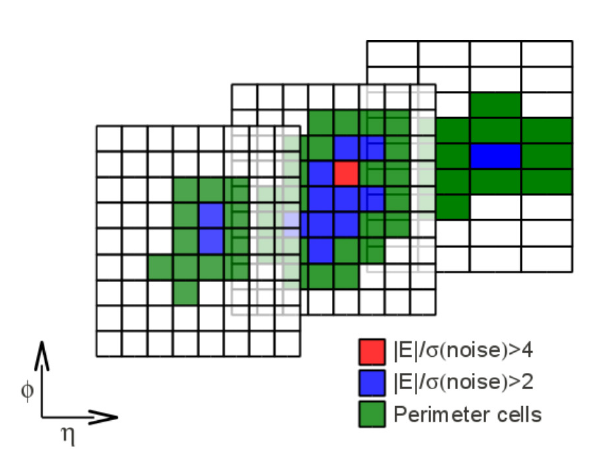
\includegraphics[width=0.65\textwidth]{figures/Objects/clusters.png}
\captionsetup{width=0.85\textwidth} \caption{\small Illlustration of the formation of a topocluster in the three hadronic layers in the barrel. The grid represents calorimeter cells.}
\label{fig:obj:jet:cluster}
\efig


\subsection{Jet finding}
Jet-finding algorithms attempt to group inputs into individual jets. To be theoretically well defined at all orders in perturbation theory, jet-finding algorithms need to be infrared-safe\footnote{If the set of inputs is modified by a soft emission, the sets of hard jets found should remain unchanged.} and collinear-safe\footnote{If the set of inputs is modified by a collinear splitting, the sets of hard jets found should remain unchanged.} \cite{Salam:2009jx}. The anti-$k_{\rm T}$ algorithm \cite{antikt} is a sequential recombination algorithm that satisfies the above conditions and that has become the most widely-used jet reconstruction algorithm at LHC. This algorithm combines iteratively two inputs into a jet based on the $\pt$-weighted distance between them, as defined in equation \ref{eq:obj:jets:d1}, and between each input and the LHC beam, as defined in equation \ref{eq:obj:jets:d2}. The algorithm defines two distances:

\be
d_{ij}= \min\left(k_{{\rm T}i}^{2p},k_{{\rm T}j}^{2p}\right)\frac{\Delta R_{ij}^{2}}{R^{2}},\,\textrm{and}
\label{eq:obj:jets:d1}
\ee

\be
d_{iB}=k_{{\rm T}i}^{2p},
\label{eq:obj:jets:d2}
\ee

\noindent where $k_{{\rm T}i}$ is the $\pt$ of input $i$, $\Delta R^{2}_{ij}= (\eta_{i}-\eta_{j})^{2} + (\phi_{i}-\phi_{j})^{2}$ is the distance squared between inputs $i$ and $j$, $R$ is a radius parameter that defines the size of the jet, and $p$ is a configurable exponent that is set to $p=-1$ for the anti-$k_{\rm T}$ algorithm. This configuration ensures that clustering is initiated by high transverse momentum objects and that the soft objects preferentially recombine with a high-$\pt$ object rather than with each other, which provides rather circular jets.
The algorithm starts by identifying the two four-vectors of an event with the smallest distance $d_{ij}$. If $d_{ij} < d_{iB}$, the two inputs are removed from the event and replaced by a single combined object, simply obtained by adding the four-momenta of the two inputs. The smallest distance $d_{ij}$  between all inputs is then recalculated, and the sequential recombination procedure continues. If $d_{iB}$ is the minimum distance then the input $i$ is designated as a final jet and removed from the event. The procedure continues until all inputs have been classified into jets. Figure \ref{fig:obj:jet:antikT} illustrates the clustering of hard and soft particles into jets when the anti-$k_{\rm T}$ algorithm is applied. The jet radius parameter $R$ defines the size of the jet and its choice is driven by the physics analysis. A larger value of  $R$ captures more of the deposited energy, particularly for particles with wide showers, while a jet reconstructed using a smaller value of  $R$ is less affected by pileup. Values of $R$ such as 0.2, 0.4 or 1.0 are common in physics analyses. The analyses described in this dissertation use anti-$k_{\rm T}$ jets with $R = 0.4$, referred to as ``small-$R$ jets''.

\bfig[h!]
\centering
\includegraphics[width=0.6\textwidth]{figures/Objects/antikT.png}
\captionsetup{width=0.85\textwidth} \caption{\small Illustration of the clustering of jets with the anti-$k_{\rm T}$ algorithm.}
\label{fig:obj:jet:antikT}
\efig

\subsection{Jet calibration}
As discussed previously, jets formed from topoclusters are reconstructed at the EM scale. The goal of the jet calibration procedure is to correct the energy of the reconstructed jets to correspond to that of the truth particle jets. This involves a series of corrections derived both from MC simulation and data, with the latter referred to as in-situ corrections \cite{ATLAS-CONF-2015-037}. The calibration scheme for calorimeter jets is illustrated in figure \ref{fig:obj:jet:JESCartoon} and described in the following sections.

\bfig[h!]
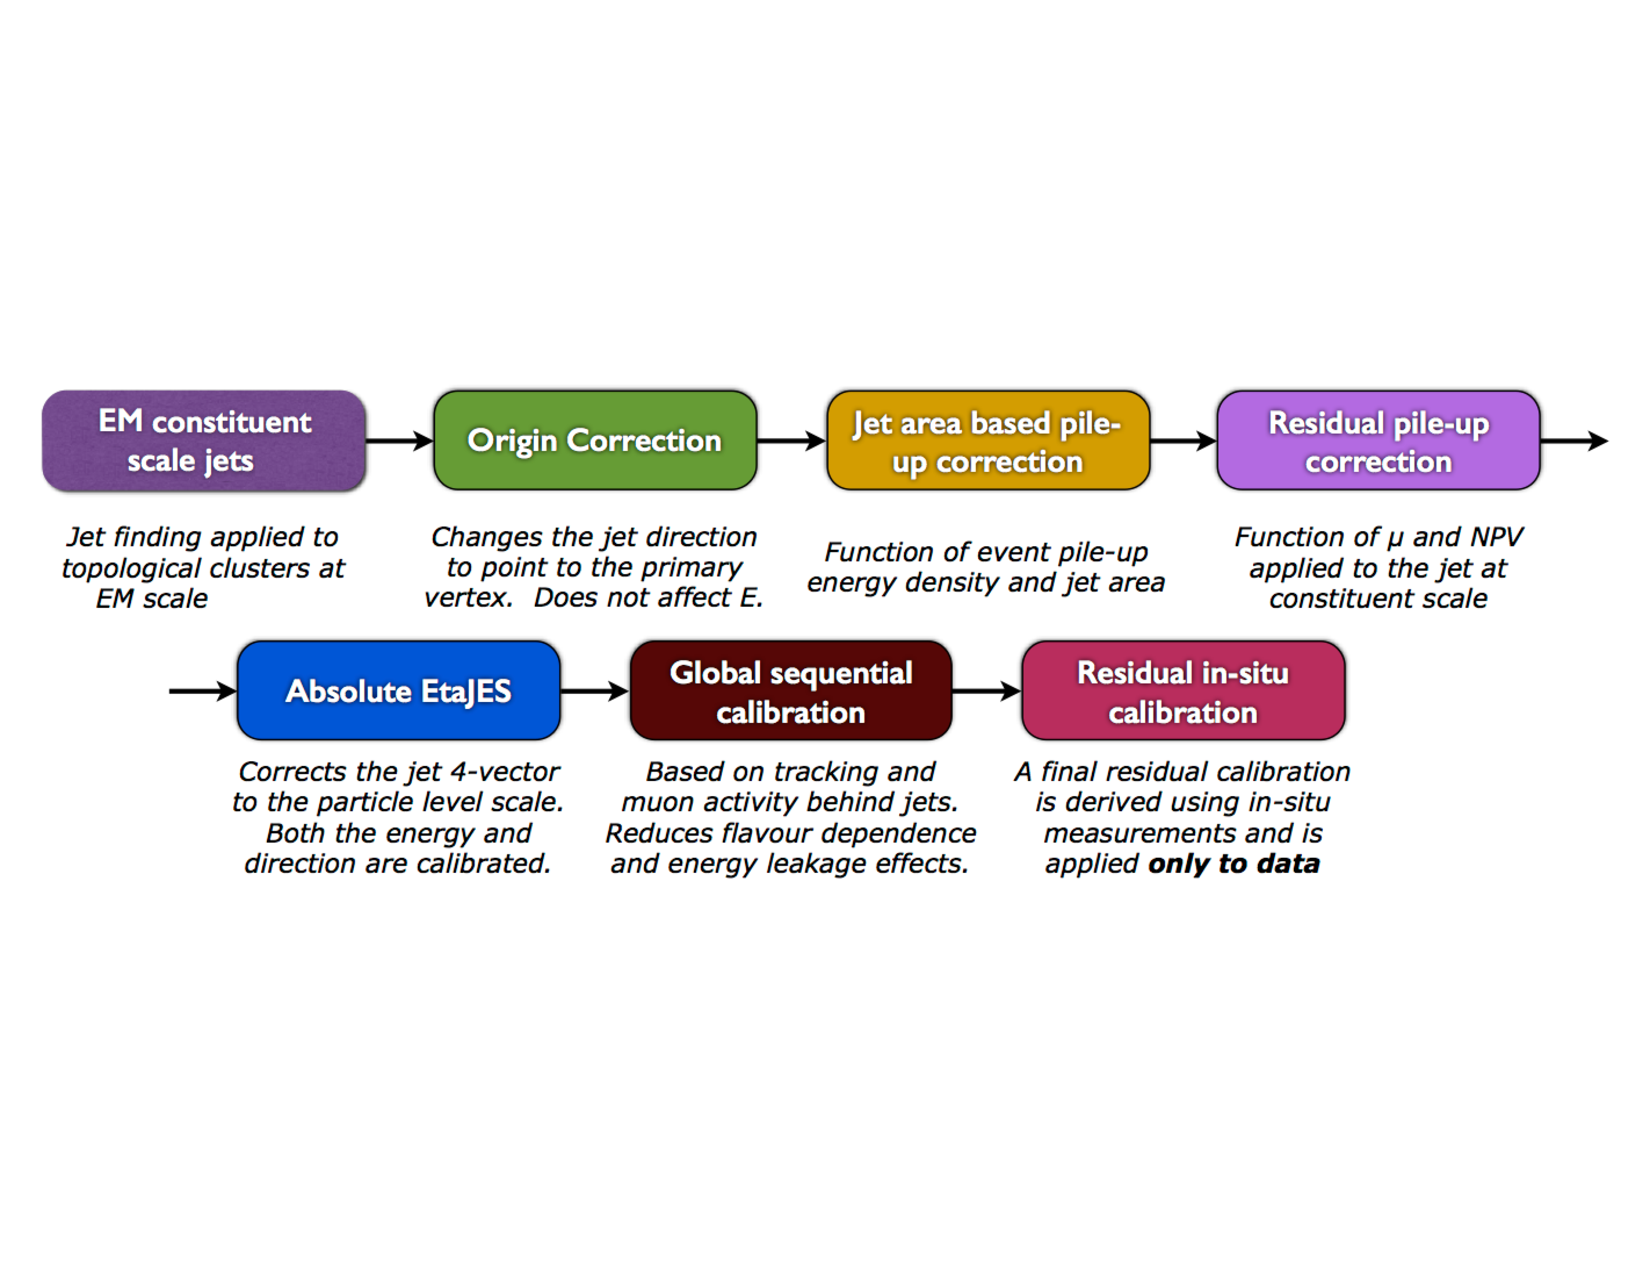
\includegraphics[width=\textwidth]{figures/Objects/JES_Cartoon.pdf}
\captionsetup{width=0.85\textwidth} \caption{\small Overview of the jet calibration procedure.}
\label{fig:obj:jet:JESCartoon}
\efig

\subsubsection{Origin correction}
The origin correction recalculates the four-momentum of jets to point to the hard-scatter PV rather than to the centre of the detector, as done by default in the clustering algorithm. This correction improves significantly the $\eta$ resolution of jets.

\subsubsection{Pileup correction}
The pileup correction accounts for additional energy deposited within the jet radius from in-time and out-of-time pileup. Pileup is assumed, on average, to deposit energy uniformly in $\eta$ and $\phi$ throughout the detector, providing a diffuse background that may be subtracted from individual jets \cite{TheATLAScollaboration:2013pia}.
The correction is performed in three steps according to this equation:

\be
\pt^{\rm corr}=\pt-\rho \cdot A -\alpha \cdot (N_{\rm PV}-1) - \beta \cdot \langle\mu\rangle,
\ee

\noindent where $\rho$ is the pileup energy density of the event based on the median energy density of jets, $N_{\rm PV}$ the number of primary vertices, $\langle\mu\rangle$ the average number of interactions per crossing, $\alpha=\frac{\partial \pt}{\partial N_{\rm PV}}$ and $\beta=\frac{\partial \pt}{\partial \mu}$. The first step represents the jet-area correction which allows a jet-by-jet estimation and subtraction of the energy added to the jet by the pileup. The area $A$ of a jet is calculated using ghost association \cite{JetArea}.\footnote{ ``Ghost'' particles of infinitesimal momentum are added uniformly to the event before jet reconstruction.} The area of a jet is determined by the number of ghost particles associated to a jet after clustering. The additional terms in the formula represent residual corrections that remove the remaining effects for both in-time ($\alpha$) and out-of-time ($\beta$) pileup. Figure \ref{fig:obj:jet:npvmudep} shows the dependence of jet $\pt$ on $N_{\rm PV}$ and $\langle\mu\rangle$ as a function of jet $|\eta|$ at various steps of the correction procedure.

\begin{figure}[t!]
\begin{subfigure}{0.5\textwidth}
  \centering
  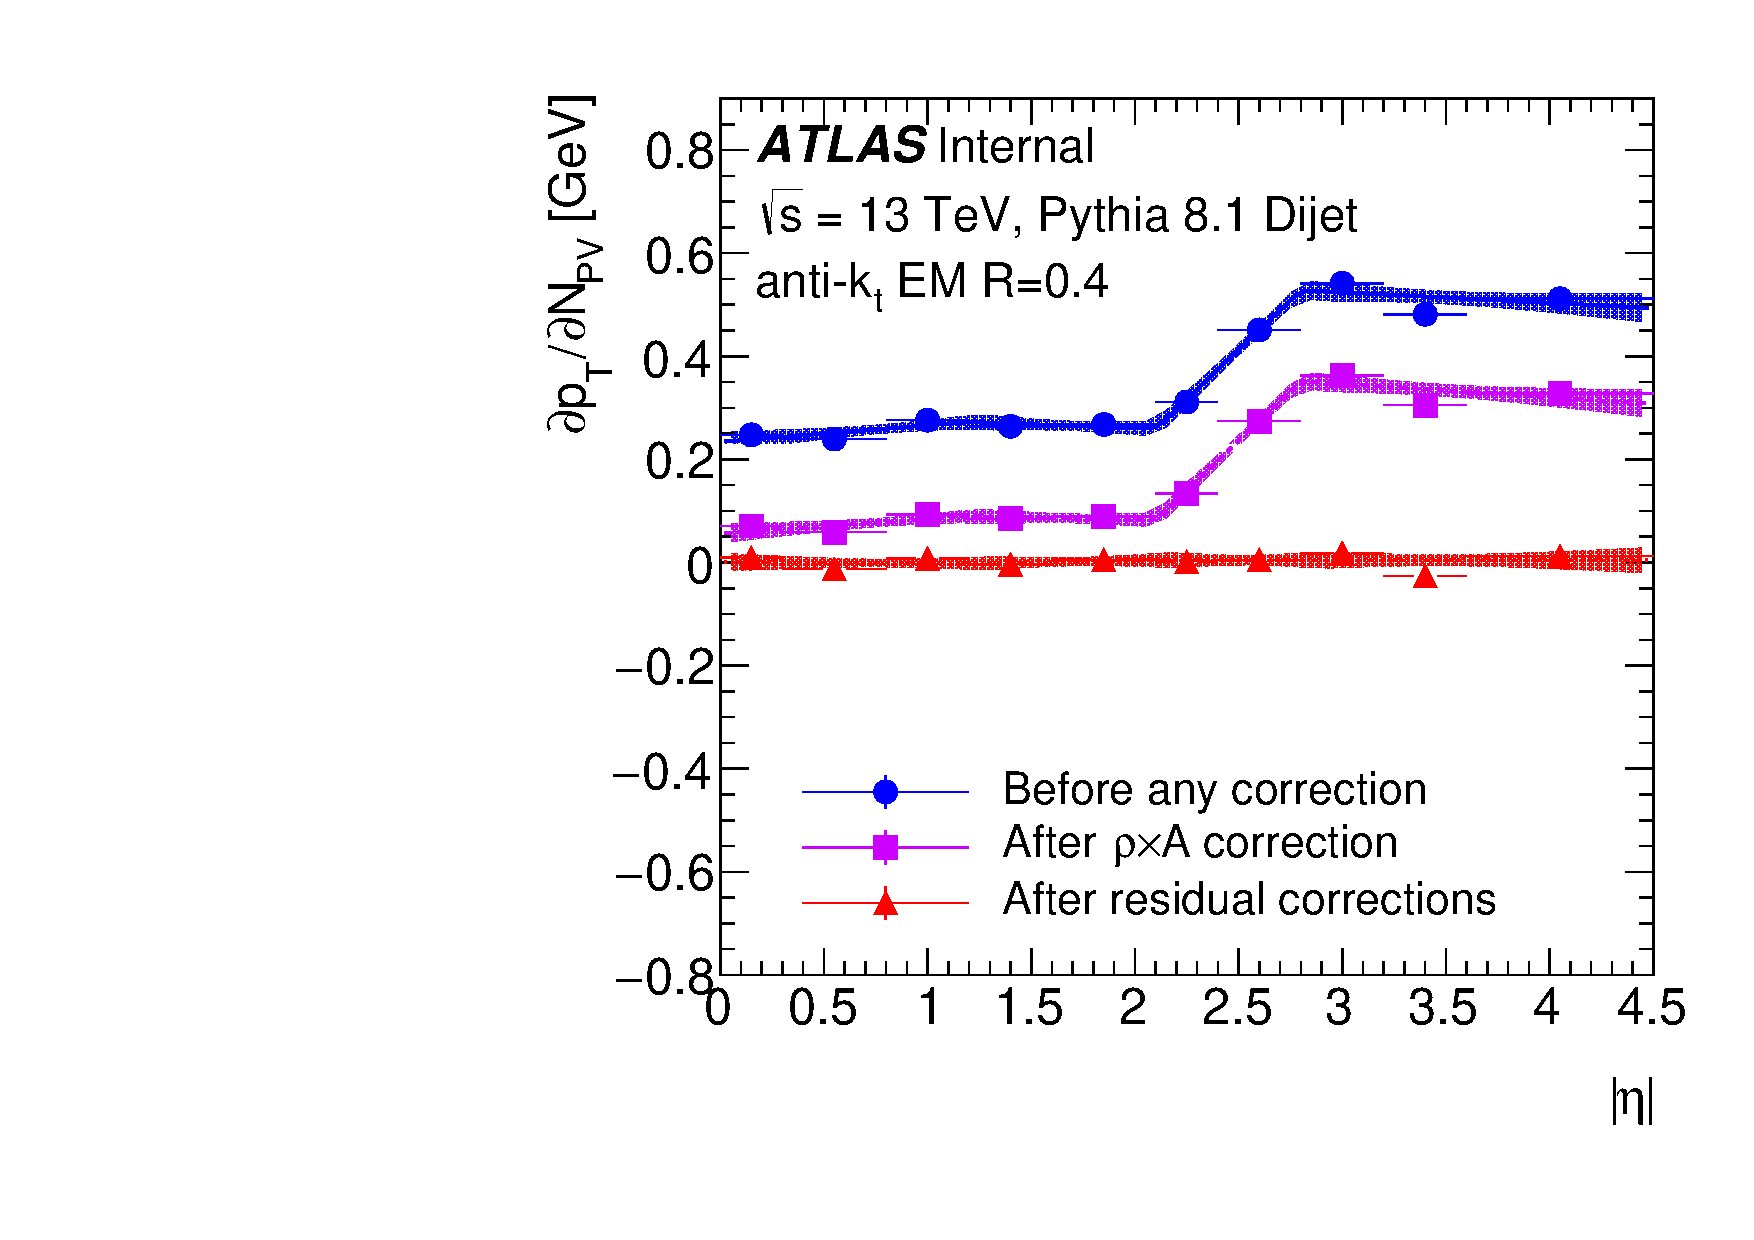
\includegraphics[width=0.9\textwidth]{figures/Objects/Pileup_EM_NPVClosure.png}
  \caption{}
  \label{fig:obj:jet:npvdep}
\end{subfigure}
\begin{subfigure}{0.5\textwidth}
  \centering
  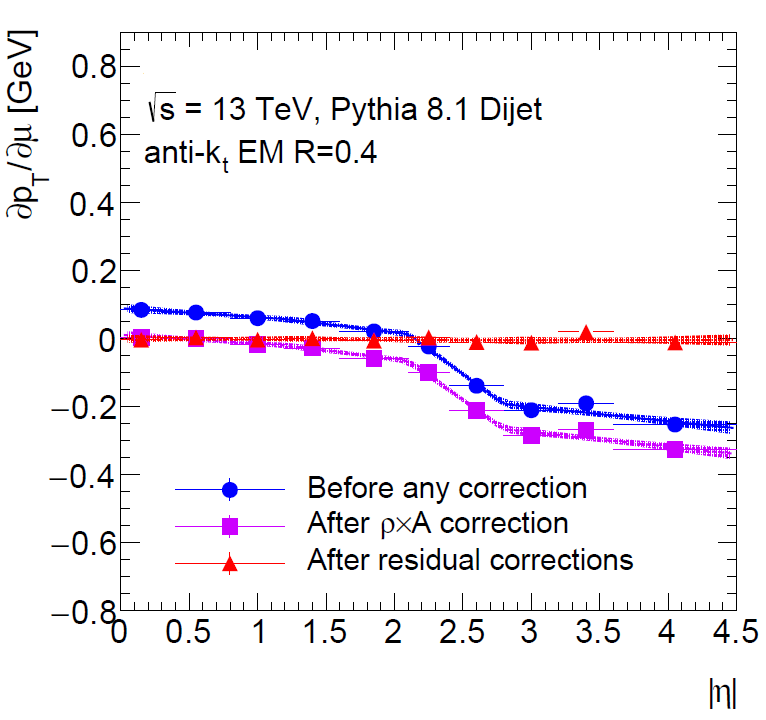
\includegraphics[width=0.9\textwidth]{figures/Objects/Pileup_EM_MuClosure.png}
  \caption{}
  \label{fig:obj:jet:mudep}
\end{subfigure}

\captionsetup{width=0.85\textwidth} \caption{\small Dependence of the reconstructed jet $\pt$ on (a) in-time pileup ($N_{\rm PV}$) and (b) out-of-time pileup ($\langle\mu\rangle$) as a function of $|\eta|$. The dependence is shown before pileup corrections (circle), after area subtraction (square), and after the residual correction (triangle).}
\label{fig:obj:jet:npvmudep}
\end{figure}

\subsubsection[Jet energy scale and $\eta$ correction]{Jet energy scale and \boldmath{$\eta$} correction}

The measured jet energy at the EM scale is lower than that at the particle level due to unmeasured energy deposited in inactive detector regions or outside of the jet radius (out-of-cone radiation), the noncompensation\footnote{Noncompensation refers to the different calorimeter response to non-electromagnetic and electromagnetic components of hadron showers.} of the hadronic calorimeters, or topocluster reconstruction inefficiencies.
After pileup correction, the jet energy scale (JES) and $\eta$ correction restores the reconstructed jet energy to the particle-level jet energy and accounts for detector effects in the jet $\eta$ reconstruction caused primarily by the transition between different calorimeter technologies and corresponding granularities. The calibration is derived from MC using isolated reconstructed calorimeter jets that are matched geometrically to truth jets within $\Delta R < 0.3$.  The ratio of reconstructed jet energy to true jet energy is parametrised as a function of the reconstructed jet's $\pt$ and $\eta$ and its inverse is applied as an energy correction. The average energy response is shown in figure \ref{fig:obj:jet:etaresp}.


\bfig[htb!]
\centering
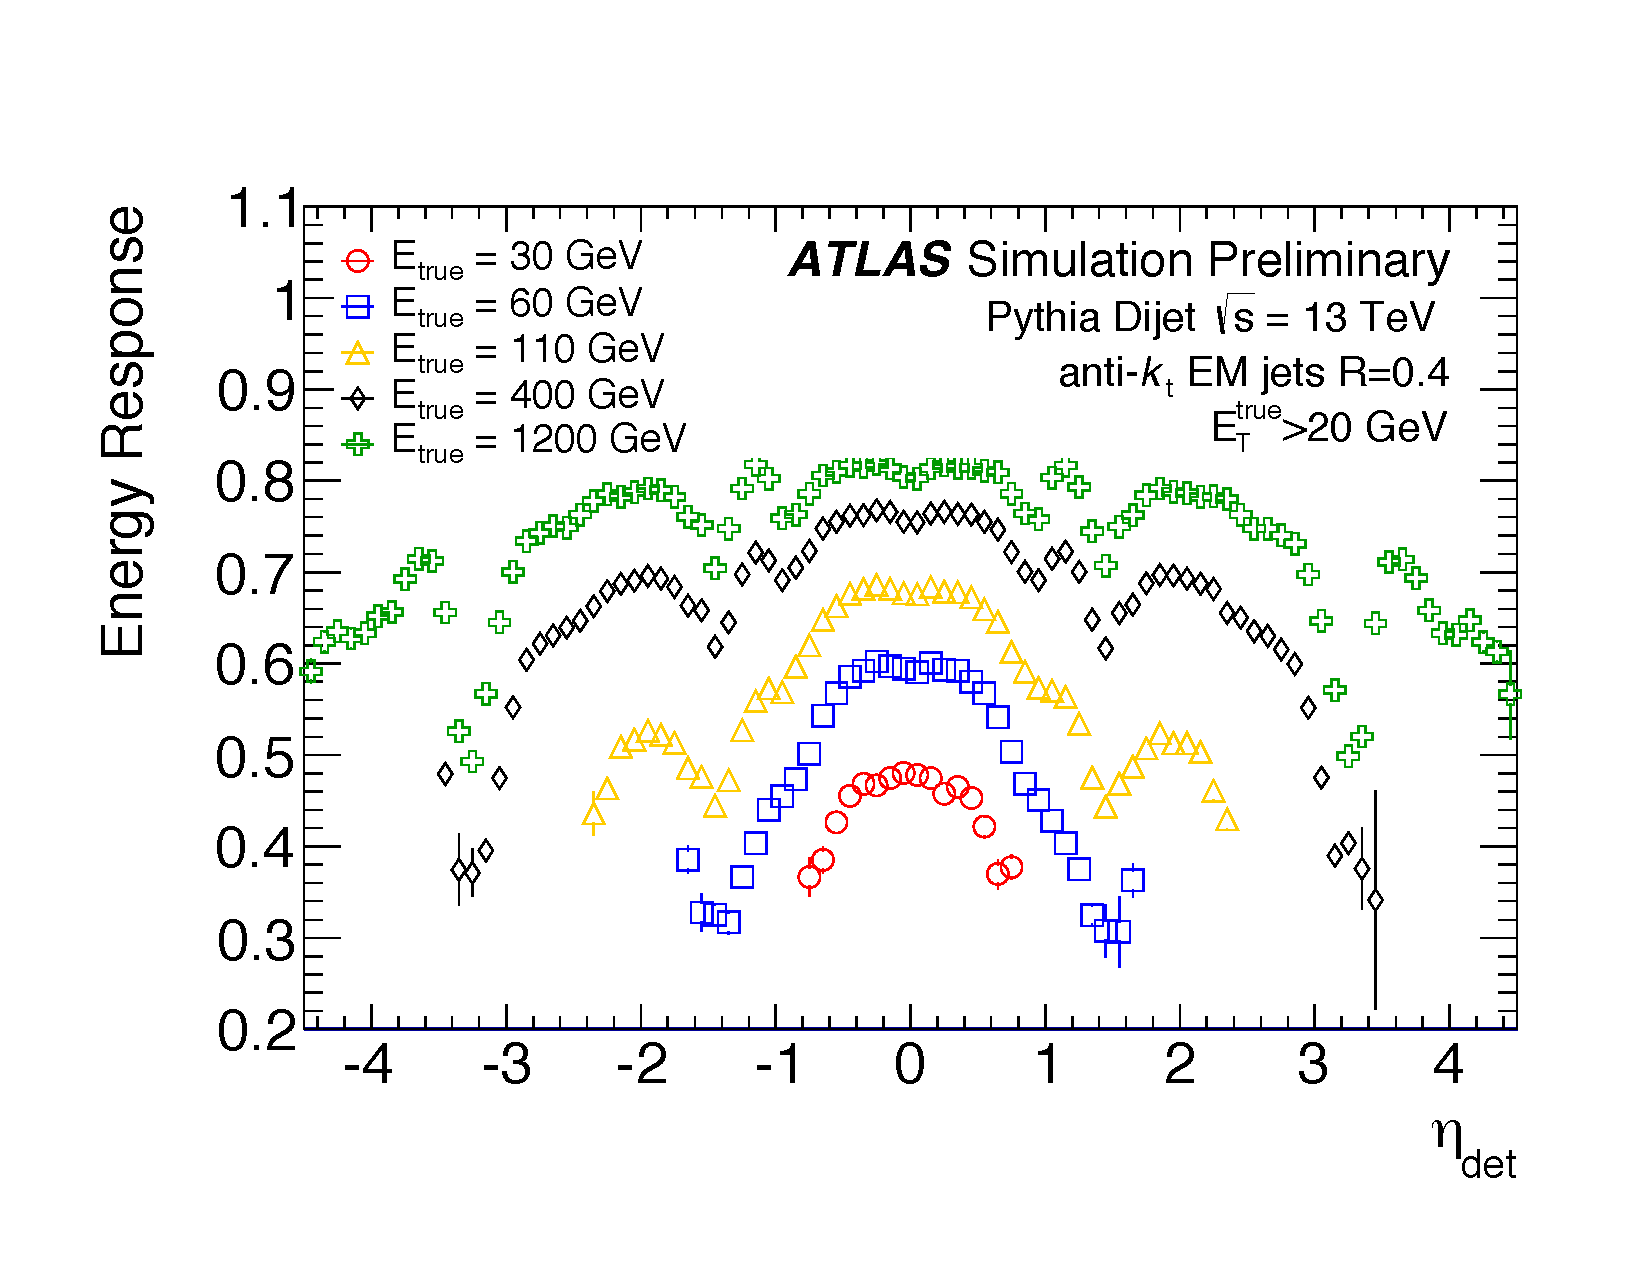
\includegraphics[width=0.7\textwidth]{figures/Objects/EtaJES_FullSim.pdf}
\captionsetup{width=0.85\textwidth} \caption{\small Average energy response for jets built from topoclusters at the EM scale. The response is shown separately for various particle-jet energies as function of the jet pseudo-rapidity $|\eta_{\rm det}|$.}
\label{fig:obj:jet:etaresp}
\efig

\subsubsection{Global sequential calibration}
The global sequential calibration is a set of independent and sequential corrections designed to remove a residual dependence of jet energy found on longitudinal and transverse features of the jet, primarily due to differences in the shower profiles between jets initiated by quarks and by gluons.  
Variables used in these corrections are:
\bi
\ib the fraction of energy measured in the first layer of the Tile calorimeter ($|\eta|<1.7$),
\ib the fraction of energy measured in the third layer of the EM calorimeter ($|\eta|<3.5$),
\ib the number of tracks associated to the jet with $\pt > 1$ $\gev$ ($|\eta|<2.5$),
\ib the width of the tracks associated with the jet, defined by the $\pt$-weighted average distance between all constituent tracks and the jet ($|\eta|<2.5$), and
\ib the number of muon segments associated with the jet ($|\eta|<2.7$).
\ei
Tracks and muon segments are associated to jets through ghost association. An additional correction, using track segments reconstructed in the muon spectrometer to identify high-$\pt$ jets that are not fully contained in the calorimeter (punch-through), is applied to reduce non-Gaussian tails in the jet response distribution. 

\subsubsection{In-situ jet calibration}
In the last step of the jet calibration differences in jet response between data and MC are quantified by balancing the $\pt$ of individual jets against well-measured physics objects. The ratio between the response in data and MC is derived as function of jet $\pt$ and $\eta$ and applied as a correction to the jets in the simulation. The in-situ techniques \cite{ATLAS-CONF-2015-037} used to derive such correction are:
\bi
\ib Dijet balance ($\eta$-intercalibration): corrects the \pt of forward jets ($0.8<|\eta|<4.5$) to that of central jets ($|\eta|<0.8$) in a dijet system, up to a $\pt$ of 1.2 $\tev$;
\ib $\gamma/Z$+jet balance: corrects the $\pt$ of central jets ($|\eta|<0.8$) to that of a well-measured photon (up to $\pt$ of 950 $\gev$) or $Z$ boson (up to $\pt$ of 260 $\gev$) in $\gamma/Z$+jet events.
\ib Multijet balance: calibrates central high-$\pt$ jets ($300 \le \pt \le 2000$ $\gev$) in events with a collection of well calibrated lower-$\pt$ jets.
\ei

Figure \ref{fig:obj:jet:respsitu} shows the ratio of the jet response as function of jet $\pt$ and $\eta$ for the three in-situ calibrations.

\begin{figure}[t!]
\begin{subfigure}{0.5\textwidth}
  \centering
  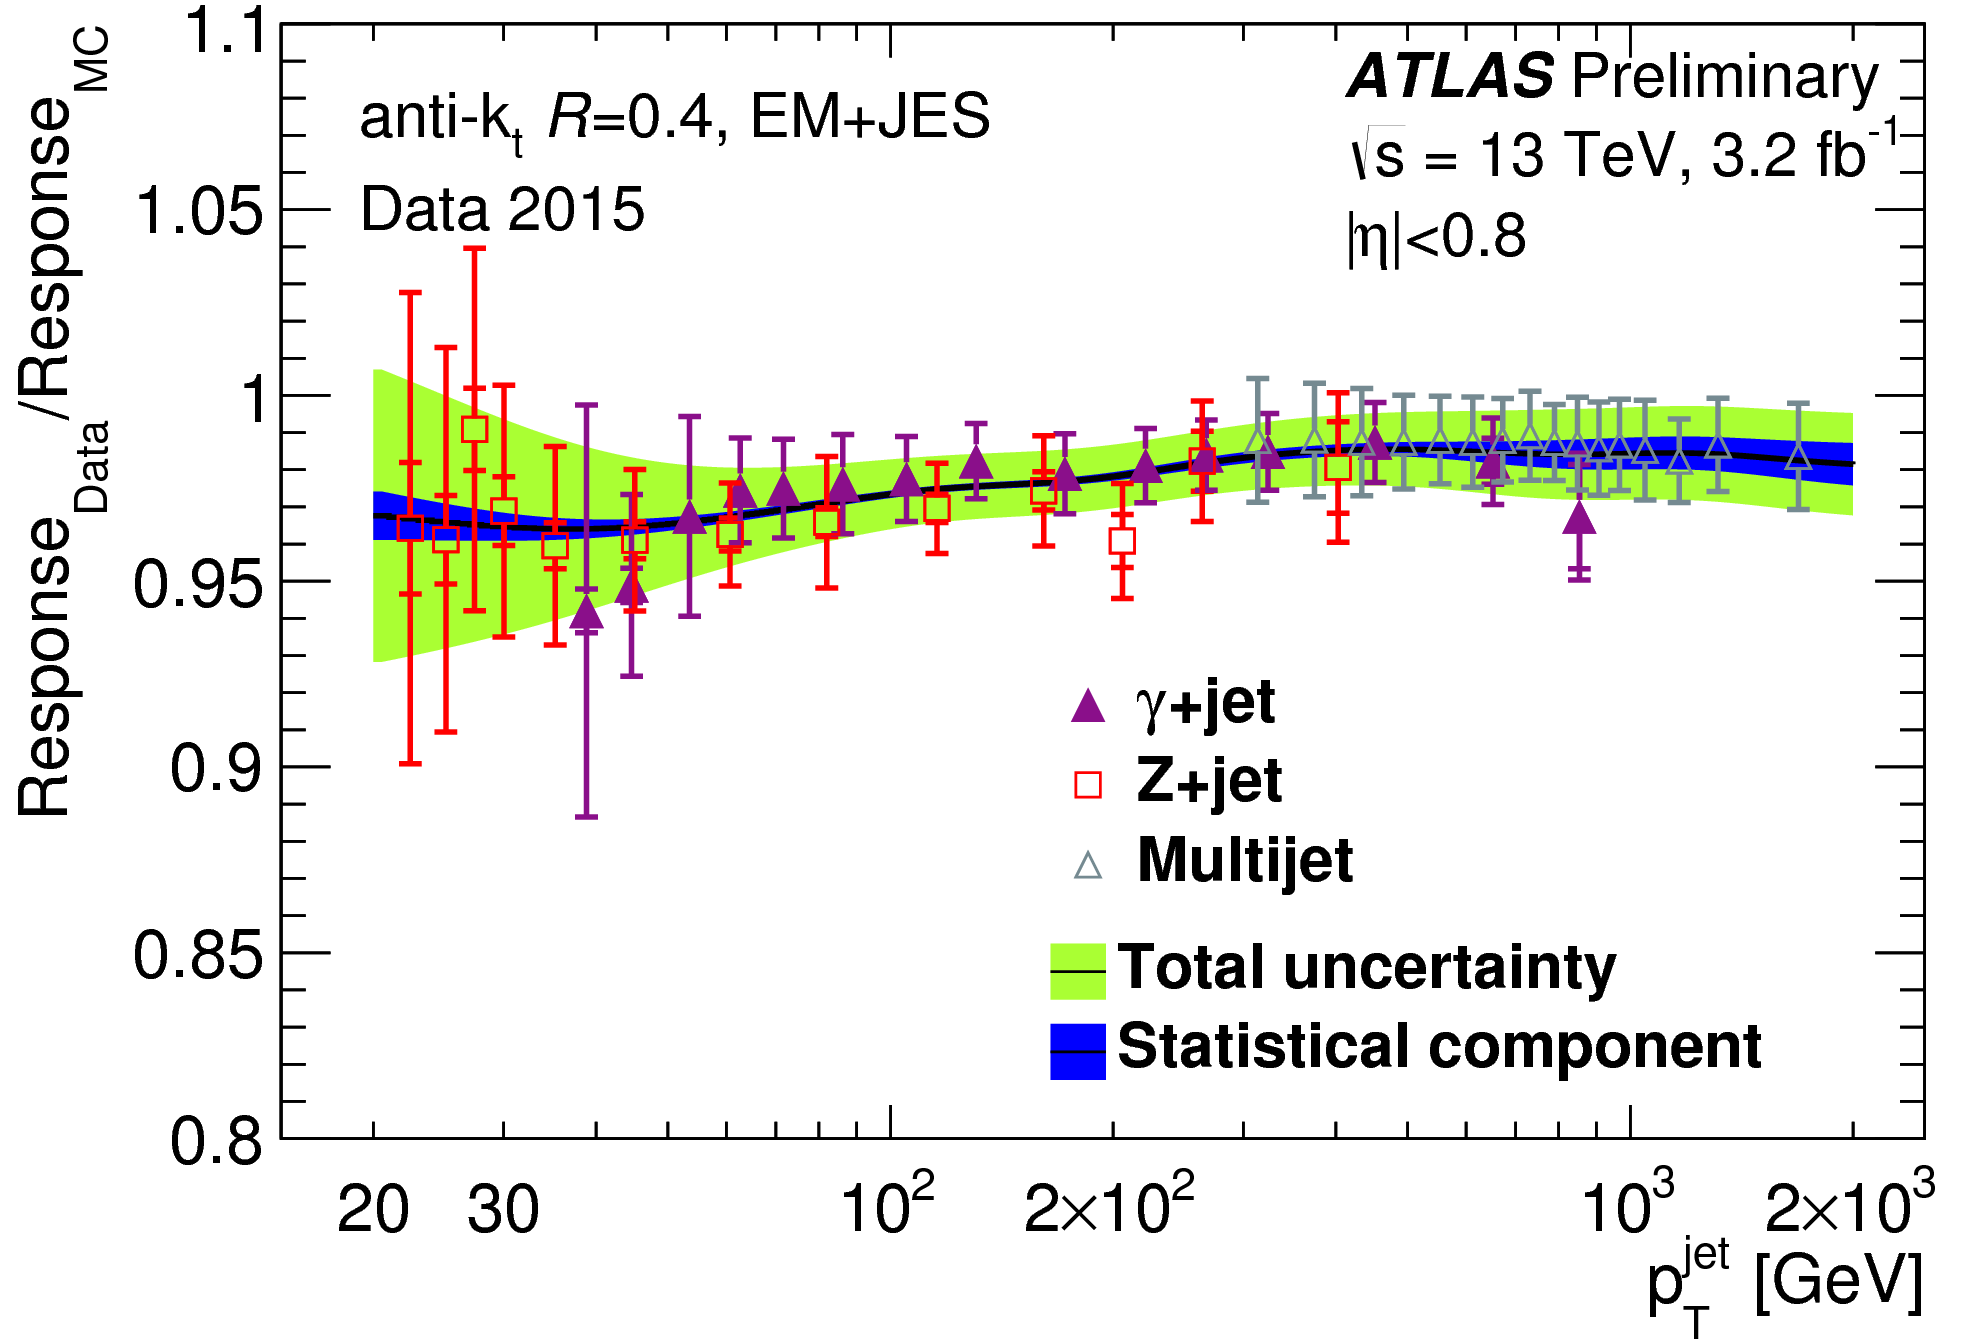
\includegraphics[width=0.9\textwidth]{figures/Objects/jetrespptsitu.png}
  \caption{}
  \label{fig:obj:jet:respsitupt}
\end{subfigure}
\begin{subfigure}{0.5\textwidth}
  \centering
  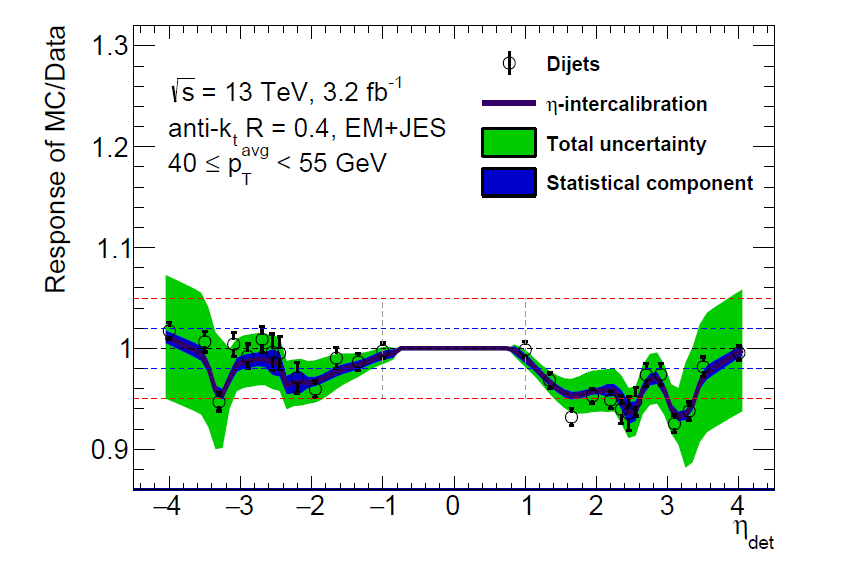
\includegraphics[width=0.9\textwidth]{figures/Objects/Combination_EIC.png}
  \caption{}
  \label{fig:obj:jet:respsitueta}
\end{subfigure}

\captionsetup{width=0.85\textwidth} \caption{\small Ratio of the average jet response in data to that measured in MC simulation (a) as a function of jet $\pt$ for different in-situ calibration techniques ($\gamma$+jet, $Z$+jet, and multijet balance) and (b) as a function of jet $\eta$ for jets with $40<\pt<55$ $\gev$ using the dijet balance technique.}
\label{fig:obj:jet:respsitu}
\end{figure}



\subsubsection{Jet energy scale uncertainties}
The JES calibration \cite{ATL-PHYS-PUB-2015-015} used in this dissertation includes a set of 19 uncertainties that takes into account multiple sources of systematic uncertainty:

\bi
\ib Four pileup uncertainties to account for potential mismodelling in the MC simulation of the number of reconstructed primary vertices $N_{\rm PV}$, the mean number of interactions per bunch crossing $\langle\mu\rangle$, and the pileup density $\rho$.
\ib Three jet-flavour-related uncertainties to account for differences in the calorimeter response and simulated jet composition of light-quark, $b$-quark, and gluon-initiated jets. In-situ techniques mainly measure quark-initiated jets by the nature of the process involved.
\ib Three uncertainties associated with the $\eta$-intercalibration technique. 
\ib Six uncertainties associated with in-situ techniques ($\gamma/Z$+jet balance and multijet balance) are divided in different categories (statistical, detector, modeling, mixed) according to their origin.
\ib One high-$\pt$ uncertainty is derived from the single-particle response and applied beyond the reach of in-situ uncertainties.
\ib One uncertainty associated with the punch-through correction applied in the global sequential calibration.
\ib One uncertainty associated with the JES correction applied to jets in the MC samples that use parametrised simulation of the calorimeter, to account for non-closure of the jet response.
\ei

Figure \ref{fig:obj:jet:jesunc} shows the relative JES uncertainty as a function of jet $\pt$ and $\eta$. The uncertainty is below $6\%$ in the whole jet $\pt$ range, reaching a value below 2\% for jets with $70<\pt<2000$ $\gev$ and $\eta=0$.


\begin{figure}[t!]
\begin{subfigure}{0.5\textwidth}
  \centering
  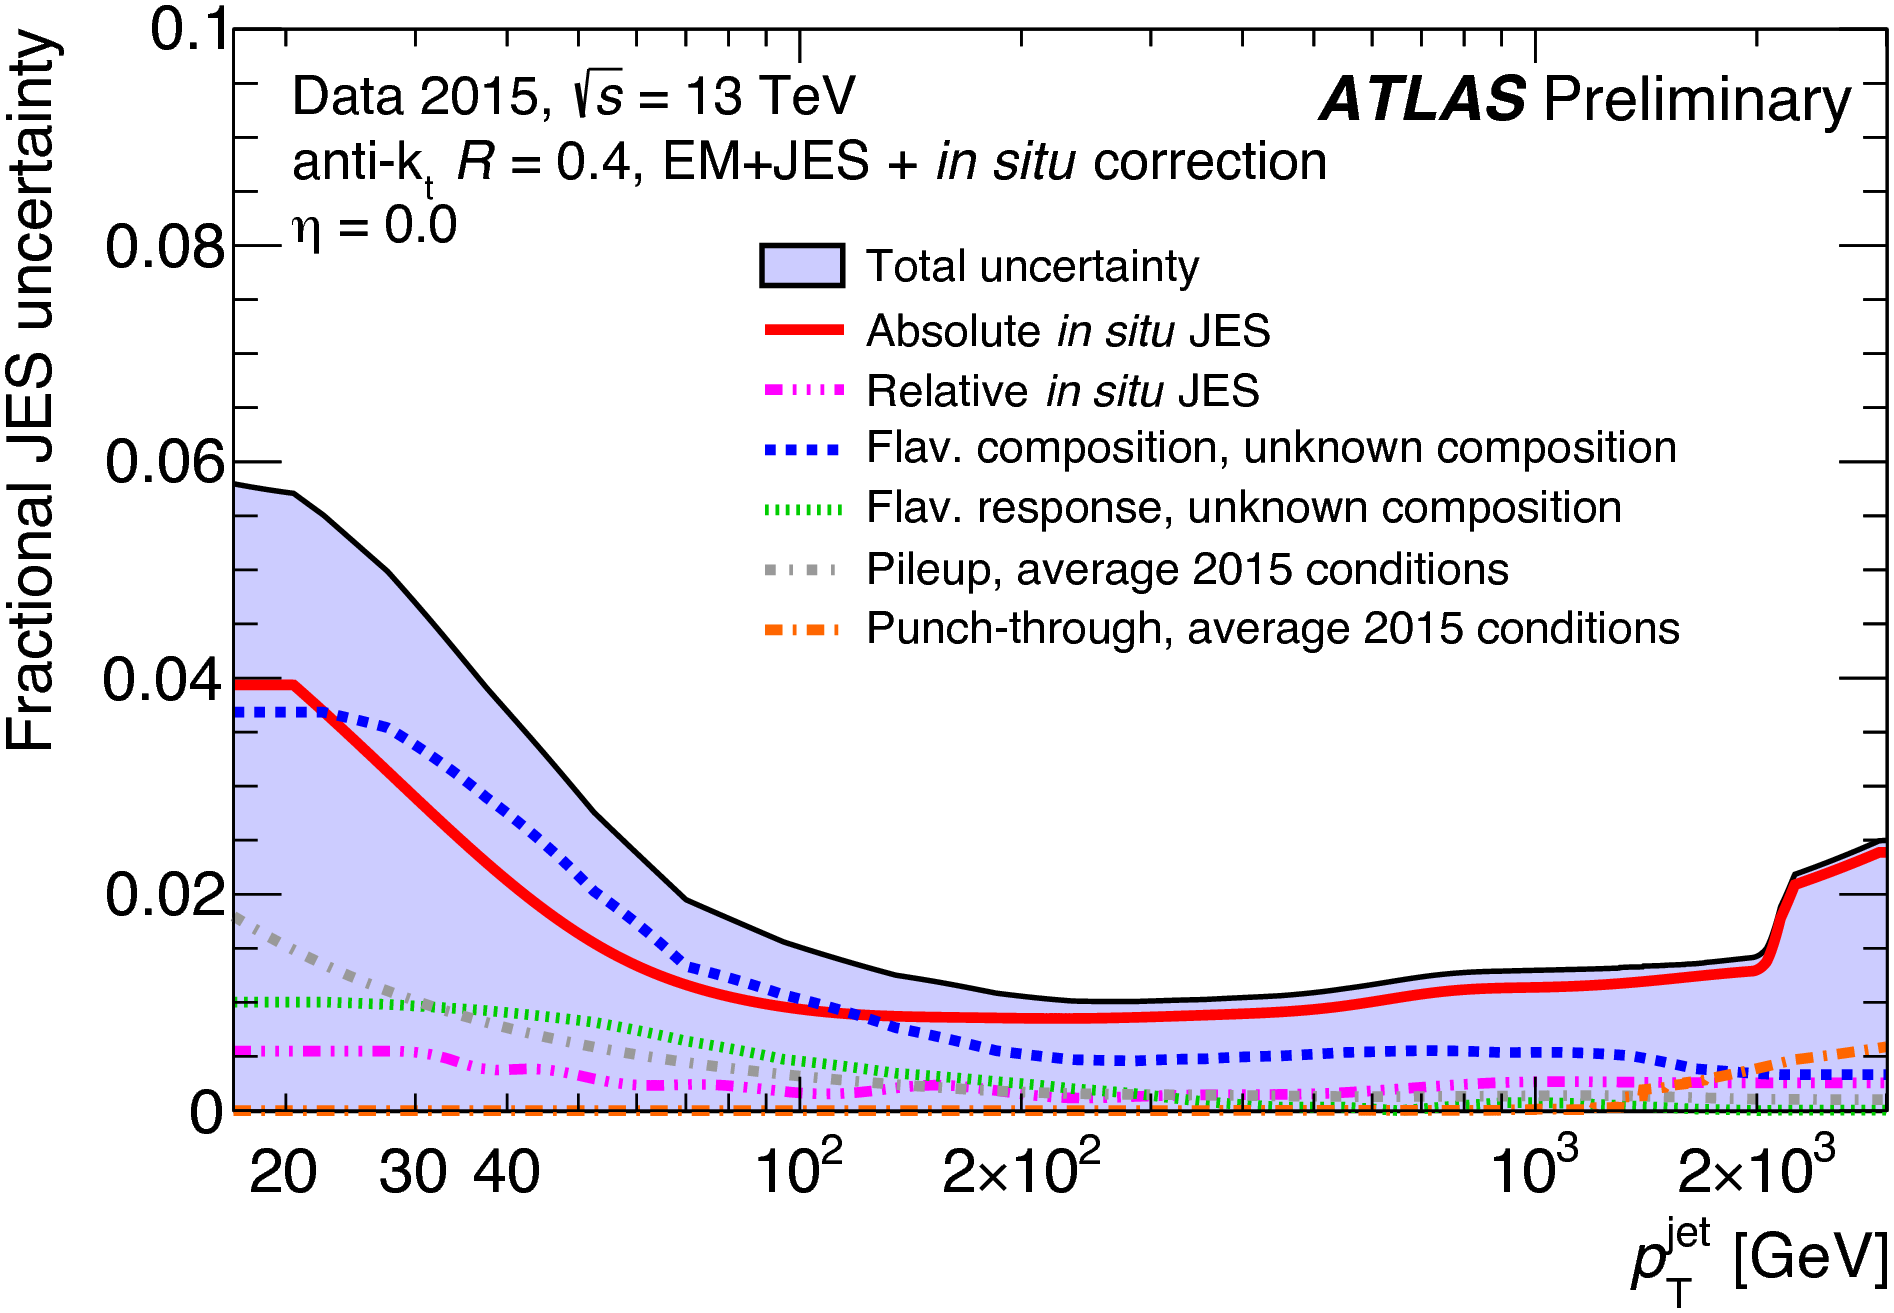
\includegraphics[width=0.9\textwidth]{figures/Objects/JESuncpt.png}
  \caption{}
  \label{fig:obj:jet:jesuncpt}
\end{subfigure}
\begin{subfigure}{0.5\textwidth}
  \centering
  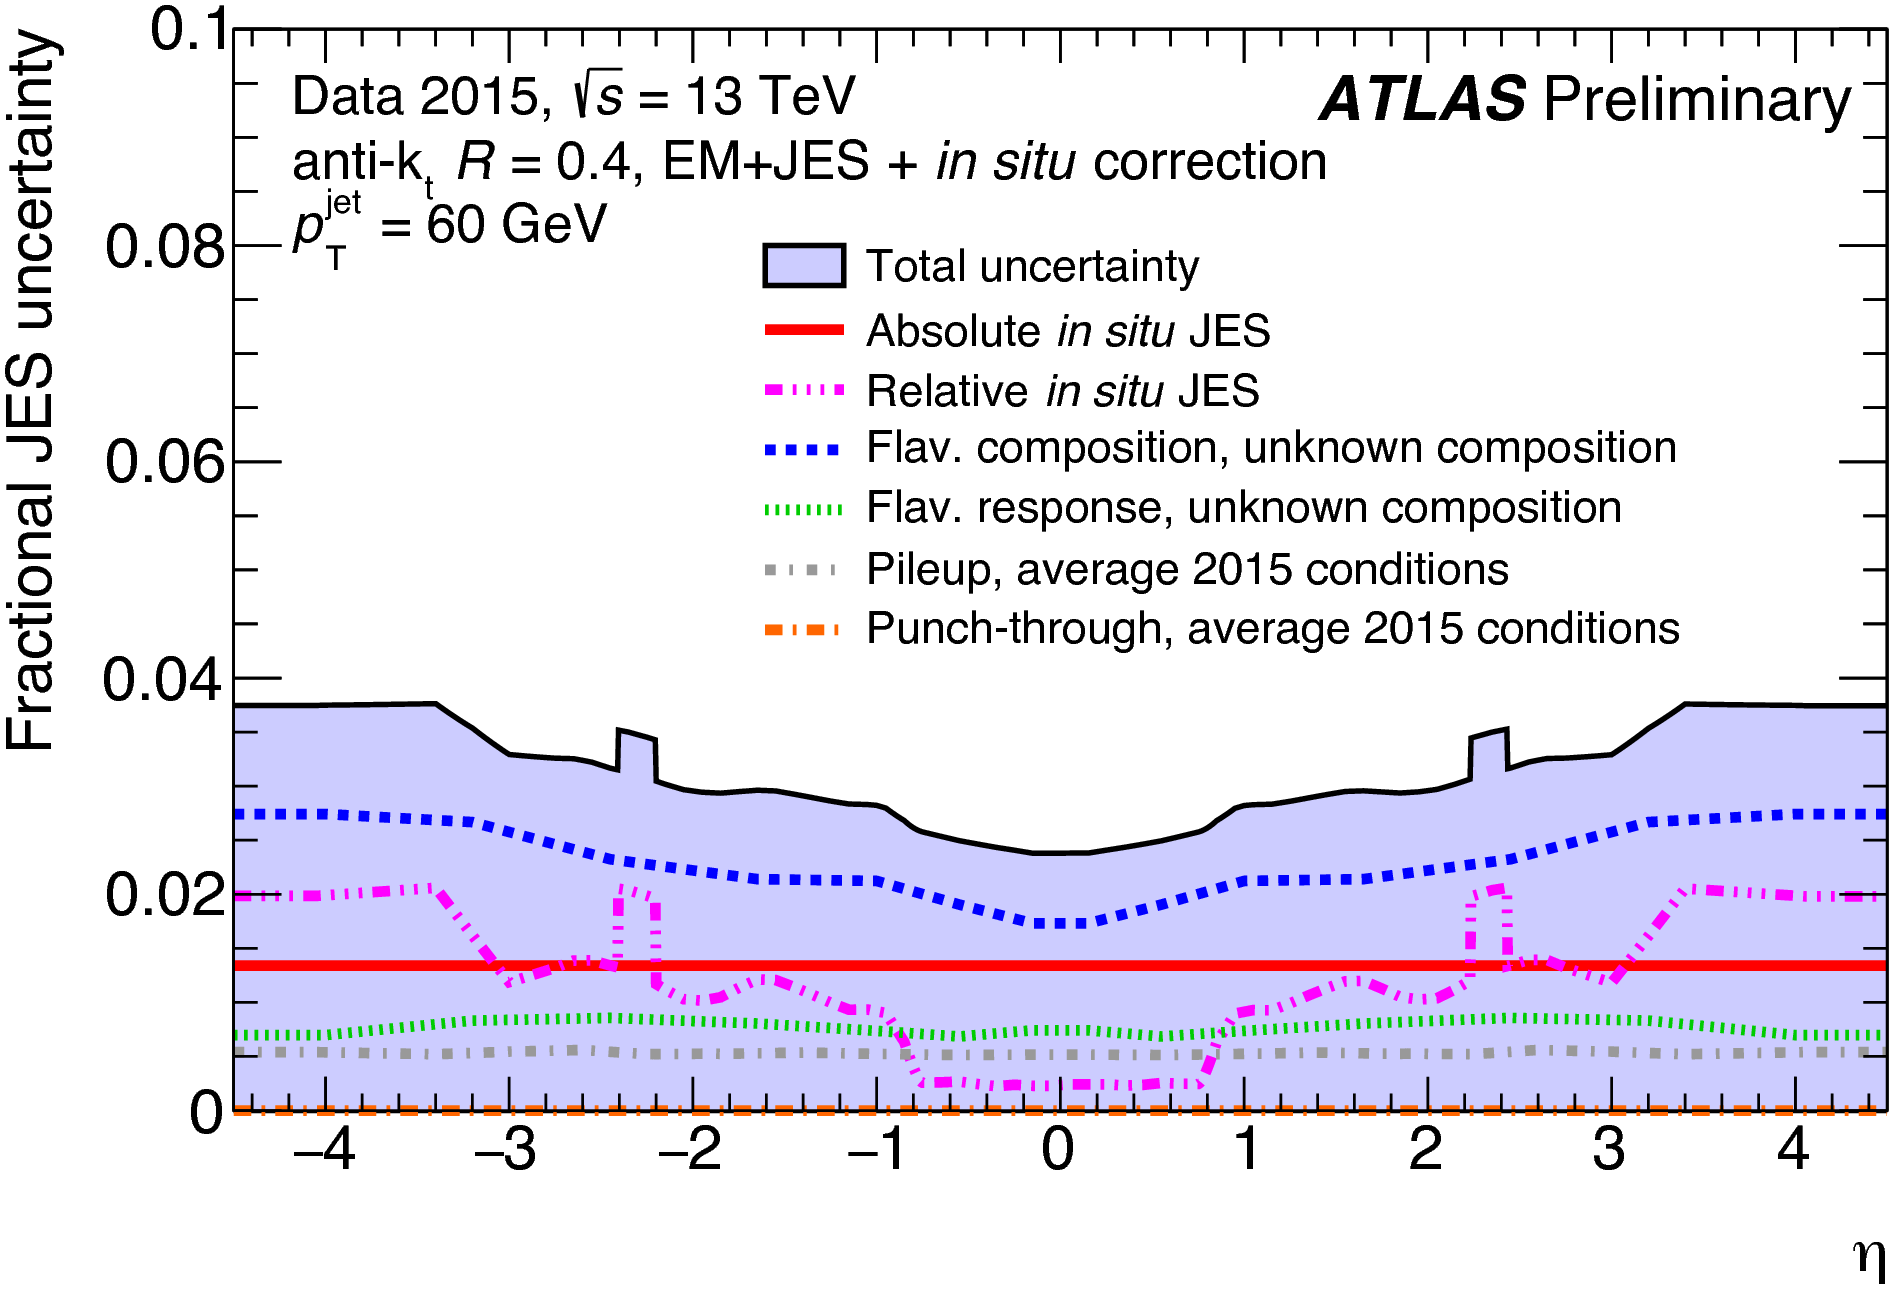
\includegraphics[width=0.9\textwidth]{figures/Objects/JESunceta.png}
  \caption{}
  \label{fig:obj:jet:jesunceta}
\end{subfigure}

\captionsetup{width=0.85\textwidth} \caption{\small Relative jet energy scale uncertainty (a) as a function of jet $\pt$ for central jets ($\eta$=0) and (b) as a function of jet $\eta$ for jets with $\pt=60$ $\gev$. The contributions from the leading sources of uncertainty are also displayed.}
\label{fig:obj:jet:jesunc}
\end{figure}

\subsubsection{Jet energy resolution}
The energy of a jet cannot be exactly measured due to electronic noise, stochastic fluctuations in the calorimeter response, and detector calibration effects. The distribution of energy measurements for jets with the same true energy is assumed to have a Gaussian shape, whose width is referred to as the jet energy resolution. The jet energy resolution in data and MC are estimated from in-situ measurements as a function of jet $\pt$ and $\eta$ \cite{ATLAS-CONF-2015-057,ATLAS-CONF-2015-017}. Figure \ref{fig:obj:jet:jer2012} shows the jet energy resolution as function of the jet $\pt$ measured using Run 1 data. Figure \ref{fig:obj:jet:jerunc} shows the estimated uncertainty on jet energy resolution as a function of jet \pt, applied to Run 2 analyses.
\begin{figure}[h!]
\begin{subfigure}{0.5\textwidth}
  \centering
  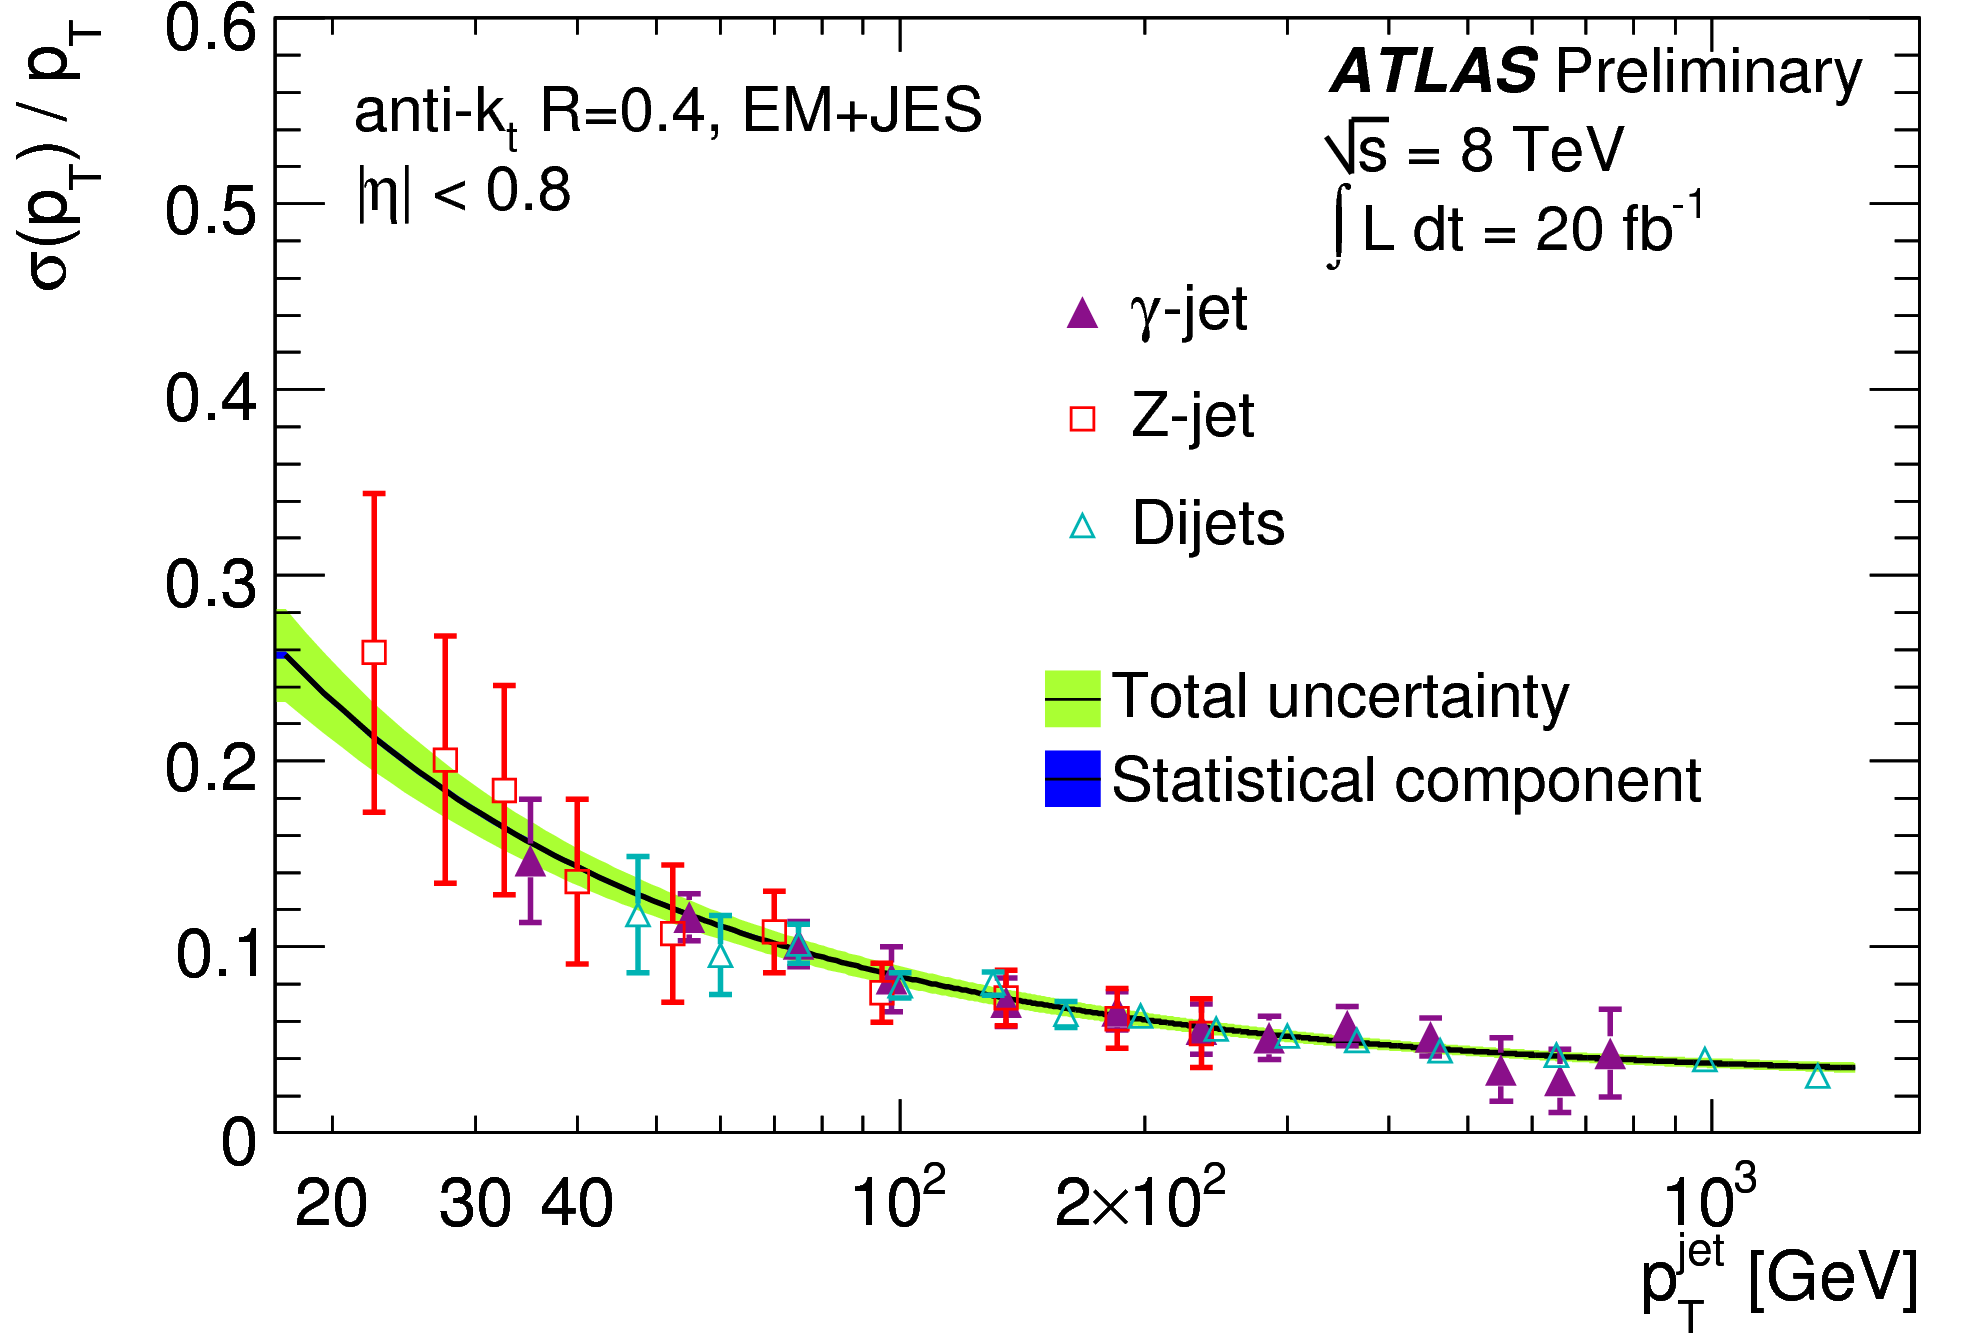
\includegraphics[width=0.9\textwidth]{figures/Objects/jer2012.png}
  \caption{}
  \label{fig:obj:jet:jer2012}
\end{subfigure}
\begin{subfigure}{0.5\textwidth}
  \centering
  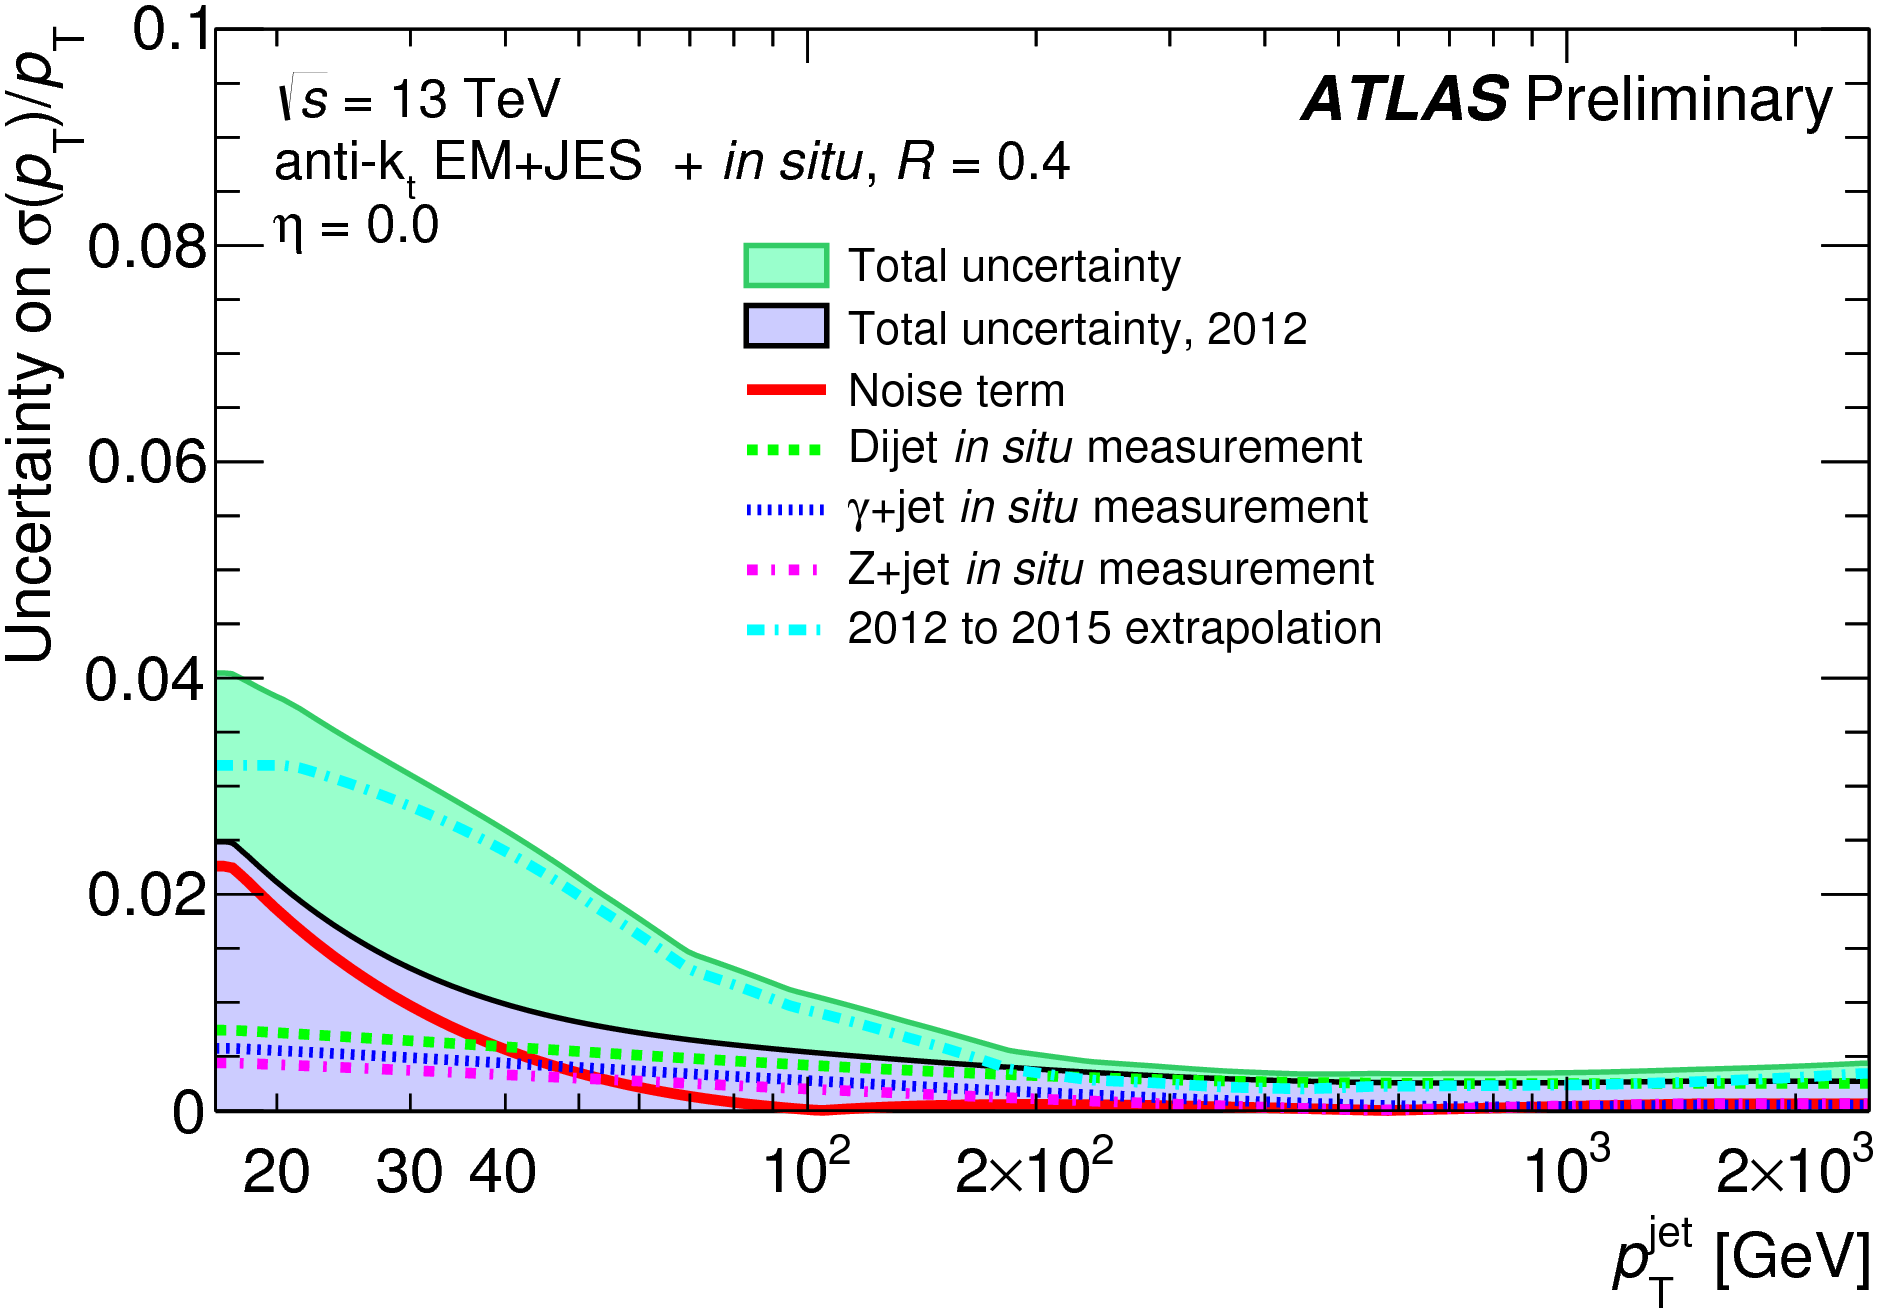
\includegraphics[width=0.9\textwidth]{figures/Objects/jeruncpt.png}
  \caption{}
  \label{fig:obj:jet:jerunc}
\end{subfigure}

\captionsetup{width=0.85\textwidth} \caption{\small (a) Jet energy resolution measurements using different in-situ techniques using Run 1 data. (b) Jet energy resolution uncertainty applied to Run 2 analyses.}
\label{fig:obj:jet:jer}
\end{figure}


\subsubsection{Jet cleaning}
\label{chp:obj:sec:jet:cleaning}
Quality criteria to reject jets not originating from $pp$ collisions (fake jets) are known as ``jet cleaning''.
Fake jets may be caused by coherent calorimeter noise that passes data quality criteria. Several sources of non-collision background may also create fake jets such as showers induced by cosmic rays or beam-gas interactions. The following quantities are used in jet cleaning:

\bi
\ib A quality factor $\mathcal{Q}_{\rm cell}$ quantitatively compares the LAr pulse to the expected pulse shape from real jets in a single cell. Jets with a significant deviation from the reference quality factor are rejected.
\ib Noise bursts in the calorimeters may also be reconstructed as negative-energy deposits. Jets with a significant absolute value of energy in all negative-energy cells (>60 $\gev$) are rejected.
\ib Energy deposits originating from calorimeter noise or beam-induced backgrounds are often localised in small regions of the calorimeter or the tracker and extend laterally in the detector rather than longitudinally. Requirements on fractions of total energy in layers of the EM calorimeter and relative fraction of jet $\pt$ measured by tracks are also used to discriminate against fake jets.
\ei
\subsubsection{Jet vertex tagger}
Pileup activity can also produce jets that should not be considered as part of the hard-scatter event. In order to identify and reject in-time pileup, information from the tracks associated to each jet is used. The Jet Vertex Tagger (JVT) \cite{ATLAS-CONF-2014-018} combines the information from two variables: corrJVF and $R_{\pt}$.\par
The corrJVF variable compares the sum $\pt$ of all tracks from the hard-scatter primary vertex (PV$_{0}$) matched to a jet, to a $N_{\rm PV}$-dependent average scalar sum $\pt$ from pileup tracks associated with a jet. It is defined as:
\be
{\rm corrJVF} = \frac{\displaystyle\sum_{i} \pt^{\rm trk_{i}} ({\rm PV}_{0})}{\displaystyle\sum_{j} \pt^{\rm trk_{j}} ({\rm PV}_{0})+\frac{\displaystyle\sum_{n\ge1} \displaystyle\sum_{j} \pt^{\rm trk_{j}} ({\rm PV}_{n})}{(k\cdot n_{\rm trk}^{\rm PU})}},
\ee
\noindent where $\sum_{i} \pt^{\rm trk_{i}} ({\rm PV}_{0})$ is the scalar $\pt$ sum of the tracks that are associated with the jet and originate from the hard-scatter vertex. The term $\sum_{n\ge1} \sum_{j} \pt^{\rm trk_{l}} ({\rm PV}_{n})$ denotes the scalar $ \pt$ sum of the associated tracks that originate from any of the pileup interactions. The factor ($k\cdot n_{\rm trk}^{\rm PU}$) with k=0.01 corrects for the linear increase of $\langle\pt({\rm PV}_{n})\rangle $ with the total number of pileup tracks per event ($n^{\rm PU}_{\rm trk}$).\par
The variable $R_{\pt}$ is defined as the scalar $\pt$ sum of the tracks that are associated with the jet and originate from the hard-scatter vertex, divided by the fully-calibrated (i.e. including pileup subtraction) jet $\pt$:
\be
R_{\pt}=\frac{\displaystyle\sum_{i} \pt^{{\rm trk}_{i}} ({\rm PV}_{0})}{\pt^{\rm jet}}.
\ee


The distribution of the JVT variable for jets originating from the hard-scatter interaction and for pileup originated jets is illustrated in figure \ref{fig:obj:jet:jvt}. The JVT variable has a good separation power between hard-scatter jets (peaking at 1) and pileup jets (having substantially lower fraction of tracks from the primary vertex, and thus peaking at 0). A value of -0.1 is assigned to jets with no associated tracks.

\bfig[t!]
\centering
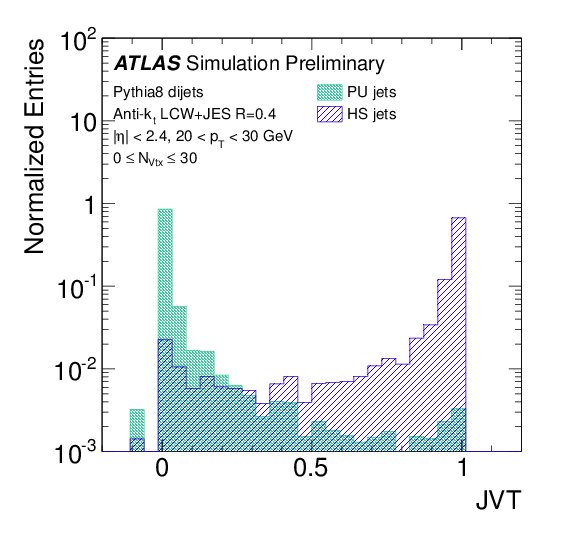
\includegraphics[width=0.5\textwidth]{figures/Objects/jvt.png}
\captionsetup{width=0.85\textwidth} \caption{\small JVT distribution for hard-scatter jets (blue shaded histogram) and pileup jets (green histogram) with $20<\pt<30$ $\gev$ and $|\eta|$<2.4 in simulated dijet events. From Ref. \cite{ATLAS-CONF-2014-018}.}
\label{fig:obj:jet:jvt}
\efig

The requirement made to suppress pileup jets is JVT > 0.59, which has a $92\%$ selection efficiency for hard-scatter jets. This cut is applied only to jets with $\pt$ < 60 GeV with $|\eta|<2.4$, since the pileup contribution at high $\pt$ is negligible. The efficiency of such cut on data and MC, and thus the corresponding SF, are derived using $Z\to \mu^{+}\mu^{-}$ events, with a selection that enriches the sample in hard-scatter jets (see figure \ref{fig:obj:jet:jvteff} ). The systematic uncertainty associated to the JVT requirement is estimated
by changing the residual contamination from pileup jets and by using different generators for the MC simulation of $Z\to \mu^{+}\mu^{-}$ events.

\bfig[h!]
\centering
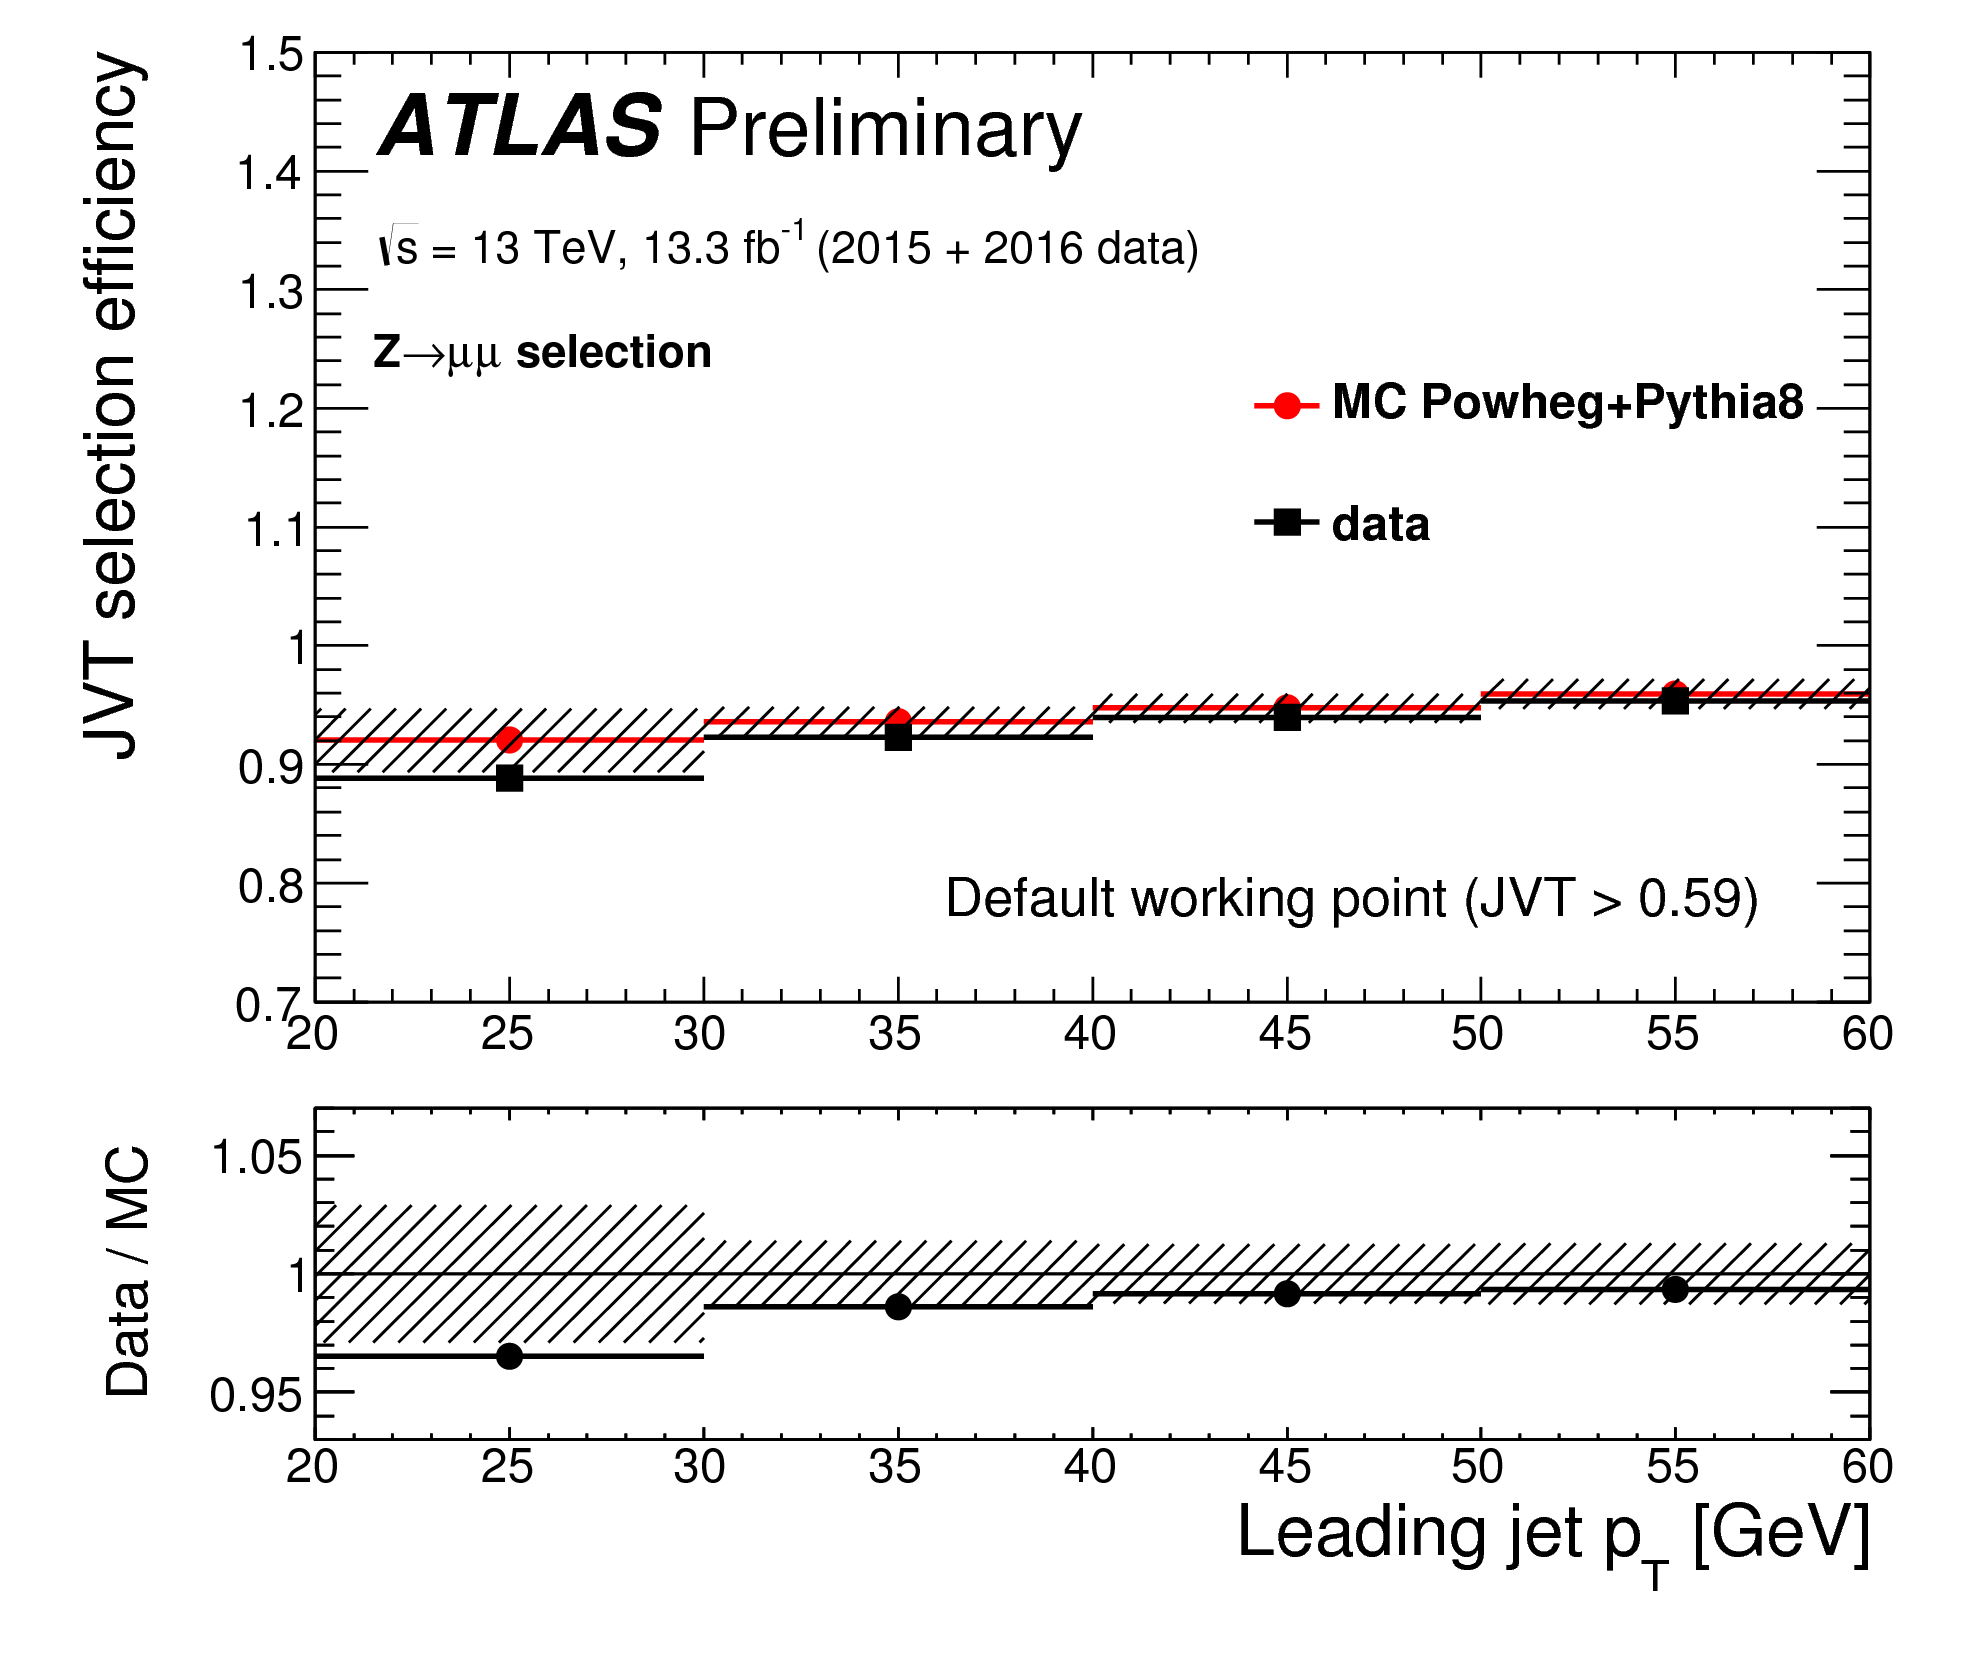
\includegraphics[width=0.6\textwidth]{figures/Objects/jvteff.png}
\captionsetup{width=0.85\textwidth} \caption{\small JVT selection efficiency for hard-scatter jets as a function of jet $\pt$, estimated in a sample of $Z\to \mu^{+}\mu^{-}$ events.}
\label{fig:obj:jet:jvteff}
\efig

\subsection{Jet re-clustering}

Processes involving the production and decay of $W$, $Z$, and Higgs bosons, as well as top quarks, provide benchmarks for testing the SM, as well as probes of physics beyond the SM. During Run 2 the  LHC operates at a centre-of-mass energy of 13 $\tev$, allowing for the first time the production of large samples of $W$, $Z$ and Higgs bosons and top quarks with a transverse momentum $\pt$ that considerably exceeds their rest mass $m$ ($\pt\gg m$).  When an unstable heavy particle is produced with such high transverse momentum (referred to as {\sl boosted object}), its decay products will become collimated in the detector frame:  the larger the boost, the closer these particles will be. The angular separation between the decay products ($\Delta R$) is approximately given by:

\be
\Delta R \approx \frac{2m}{\pt},
\ee

\noindent where $m$ and \pt are respectively the mass and the transverse momentum of the unstable heavy particle.\\
Figure \ref{fig:obj:jet:boostdr}  illustrates the dependence of $\Delta R$ between the decay products of a top quark as a function of top-quark $\pt$.

\bfig[htb!]
\centering
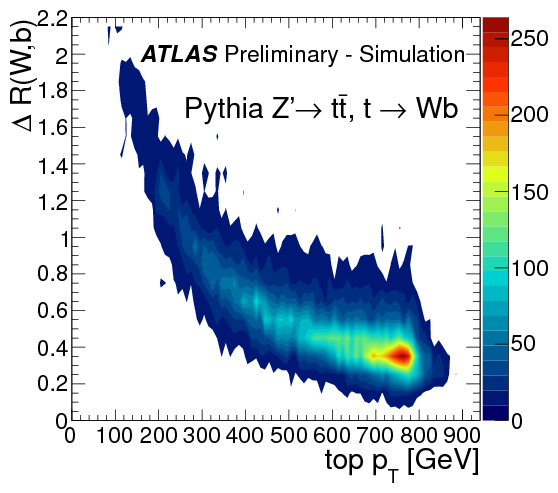
\includegraphics[width=0.6\textwidth]{figures/Objects/boostdr.png}
\captionsetup{width=0.85\textwidth} \caption{\small Angular separation between the decay products of a boosted top quark from a heavy $Z^{`}\to t\bar{t}$, as a function of top-quark $\pt$ .}
\label{fig:obj:jet:boostdr}
\efig

In the case of hadronic decays of boosted objects, the pairs or triplets of conventional $R=0.4$ anti-$k_{\rm T}$ jets that would normally be used to reconstruct the heavy particle (resolved regime), may be close enough that it is instead possible to reconstruct the system using a single large-radius (large-$R$) jet (boosted regime), as shown in figure \ref{fig:obj:jet:boostcart}.

\bfig[t!]
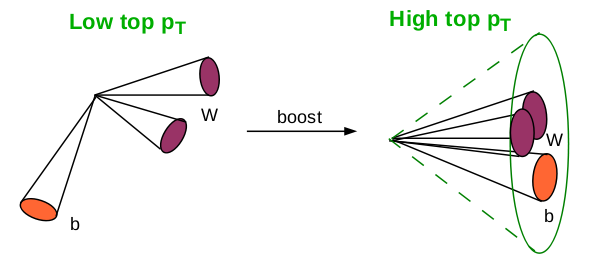
\includegraphics[width=\textwidth]{figures/Objects/cartoonboost.png}
\captionsetup{width=0.85\textwidth} \caption{\small Graphical representation of resolved (left) and boosted (right) topologies.}
\label{fig:obj:jet:boostcart}
\efig

In the boosted regime, the masses of jets and further details of the jet substructure will be useful in identifying single jets from hadronic decays of boosted objects from those originating from QCD processes (e.g. the jet mass will peak around the resonance mass). A variety of tools are proposed to identify resonances using different substructure observables and algorithms to build large-$R$ jets \cite{Altheimer:2013yza}. The larger radius makes large-$R$ jets more susceptible to pileup effects. Therefore, several techniques (``grooming'') have been developed to suppress the pileup or underlying-event contaminations affecting large-$R$ jets:

\bi
\ib Trimming \cite{Krohn:2009th}: In this approach the constituents of the large-$R$ anti-$k_{\rm T}$ jet are re-clustered  into smaller jets with $R_{\rm trim}= 0.2$, using the anti-$k_{\rm T}$ algorithm again. The resulting subjets are only accepted if their transverse momentum is larger than a fraction $f$ (here $f= 0.03$) of a hard scale, which is chosen to be the $\pt$ of the large-$R$ jet. The surviving subjets are recombined into a groomed jet.
\ib Filtering \cite{Butterworth:2008iy}: The procedure is similar to trimming, except that in this case the subjets are found with the Cambridge-Aachen algorithm \cite{antikt} with $R_{\rm filt}= 0.3$, and only the three highest-$\pt$ subjets are  retained.  The groomed jet is then constructed from these three subjets.
\ib Pruning \cite{Ellis:2009su}: Contrary to trimming and filtering, this procedure is applied during jet finding.  It dynamically suppresses soft and large-distance contributions to the jet
using two parameters, $Z_{\rm cut}$ for the momentum-based suppression, and $D_{\rm cut}$ for the distance-based suppression. Pruning vetoes recombinations between two objects $i$ and $j$ for which $\Delta R_{ij}> D_{\rm cut}$ and if the $\pt$ of one of the objects is less than $Z_{\rm cut}\times \pt^{ij}$, where $\pt^{ij}$ is the combined transverse momentum of $i$ and $j$. In this case, only the hardest (highest \pt) of the two objects is kept. Typical values for these parameters are:  $D_{\rm cut}=0.5$ and $Z_{\rm cut}=0.1$.
\ei

 In this dissertation only one method to build large-$R$ jets will be discussed, referred to as ``jet re-clustering'' \cite{Nachman:2014kla}. Jet re-clustering takes as inputs small-radius ($R\le0.4$) jets and clusters them into large-radius ($R\ge1.0$) jets. The calibrations, corrections, and uncertainties on the re-clustered jets are inherited from the small-$R$ jets, so this method solves difficulties in calibration and uncertainty estimation.
By construction, re-clustered jets are already groomed to some extent. Small-$R$ jets can only be calibrated to some low $\pt$ value (typically 20 $\gev$) and thus effectively ``subjets'' are removed that are below this fixed $\pt$ threshold. To improve the performance of the re-clustered jet mass reconstruction, further grooming can be applied. In particular, re-clustered trimmed jets (RT-jets) are subject to the removal of all small-$R$ jets within the re-clustered jet with \pt below $f_{\rm cut}\times \pt^{\text{\rm re-clustered jet}}$, in analogy to standard large-$R$ jet trimming.  However, re-clustered trimming differs in an important way:  the jet \pt of the re-clustered jet and its subjets are calibrated, including pileup correction.
In Figure \ref{fig:obj:jet:RTmass}, the mass distribution of re-clustered jets and RT-jets are compared for simulated $Z^{\prime}\to t\bar{t}$ events. In the case of the RT-jets, clear peaks are visible around the $W$-boson and top-quark masses with a performance comparable to that of standard large-$R$ trimmed jets.

\bfig[t!]
\centering
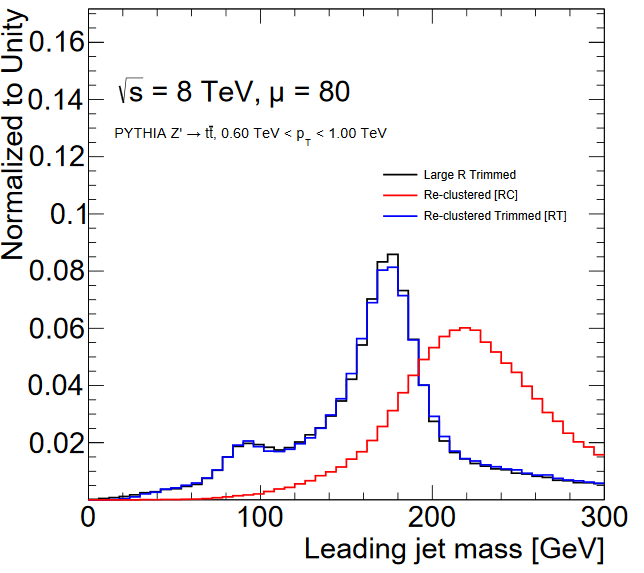
\includegraphics[width=0.5\textwidth]{figures/Objects/RTmass.png}
\captionsetup{width=0.85\textwidth} \caption{\small Mass distribution for different large-$R$ jets. The jet mass performance for re-clustered large-$R$ jets is comparable to that of standard large-$R$ jets only after trimming. In this figure a value of $\langle\mu\rangle$ much higher than that expected in Run 2 is assumed to check the performance in extreme conditions.}
\label{fig:obj:jet:RTmass}
\efig

The usual approach to jet substructure is to build large-$R$ jets and then look inside the jet for structure on finer angular scales (top-down substructure). Re-clustered jets inherit this approach by associating the small-$R$ jet constituents to the large-$R$ jets, and then computing substructure variables as usual. However, an advantage of re-clustered jets is that some substructure variables can be computed using a bottom-up approach, in the sense that they are constructed from the the kinematics of the small-$R$ jets themselves, and thus are a-priori corrected and calibrated.  In order to ensure that the mass of the large-$R$ jet originates from the $\pt$ and angular separation of the subjets, instead of from the small-$R$ jet mass (that at the time of this writing is not calibrated yet), a requirement of at least two subjets is made.  In this way it is possible to evaluate the uncertainty on the mass of the large-$R$ jets coming from the calibration of its constituents by varying the energy scale and resolution of small-$R$ jets.

The analyses described in this dissertation use anti-$k_{\rm T}$ RT-jets from small-$R$ jets ($R=0.4$) with a radius of $R=1.0$, which are trimmed  by removing all small-$R$ jets within a re-clustered jet that have $\pt$ below $5\%$ of the $\pt$ of the re-clustered jet (i.e. $f_{\rm cut}=0.05$).  Due to the pileup suppression and $\pt>25$ $\gev$ requirements made on the small-$R$ jets, the average fraction of small-$R$ jets removed by the trimming requirement is less than $1\%$.  



\subsection[$b$-tagging]{\boldmath{$b$}-tagging}
\label{sec:obj:jets:btagging}
The identification of jets resulting from the fragmentation of $b$-quarks ($b$-jets), usually referred to as $b$-tagging, is of crucial importance in event topologies involving $b$-quark such as those with top-quark of $H \to b\bar{b}$ decays.\par
Jets produced in the hadronisation of $b$-quarks can be distinguished from other types of jets using the characteristic properties of $b$-hadrons (see figure \ref{fig:obj:jet:btagip}).
\bfig[t!]
\centering
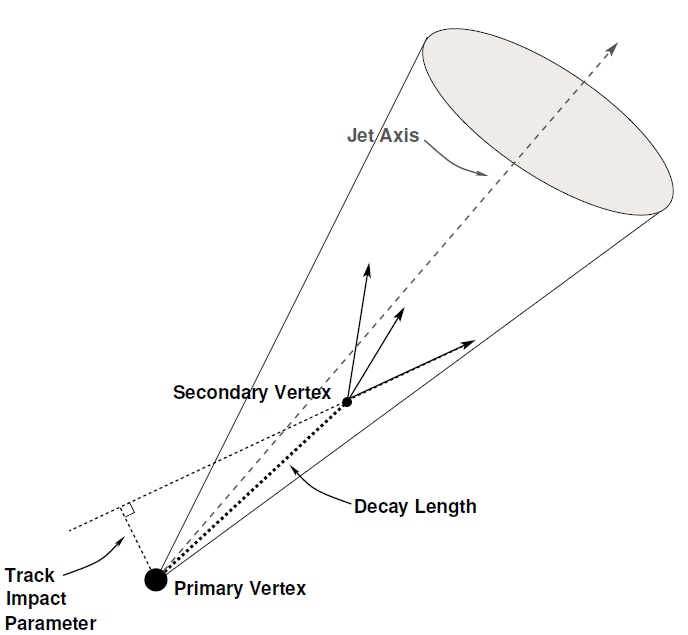
\includegraphics[width=0.5\textwidth]{figures/Objects/btagip.png}
\captionsetup{width=0.85\textwidth} \caption{\small Most relevant variables for the identification of $b$-jets.}
\label{fig:obj:jet:btagip}
\efig
Because of their long lifetime ($\tau\sim1.5$ ps, $c\tau \sim450$ $\mu$m) $b$-hadrons can travel several millimetres before decaying producing at least one displaced vertex in the jet, which can be reconstructed. Also, it is possible to measure the impact parameters of the tracks from the $b$-hadron decay products, which tend to have rather large positive impact parameters and thus can be distinguished from tracks coming from the primary vertex. The sign of the impact parameter is positive if the track extrapolation crosses the jet direction in front of the primary vertex, and negative otherwise. For a jet originating from a $b$-quark, typically one or more tracks are expected to show a large and positive impact-parameter significance, defined as the impact parameter over its error. Negative impact parameters typically occur because of resolution effects. The longitudinal and transverse impact parameters are defined as the minimum distance of the track to the primary vertex respectively in the $z$ direction and in the $x-y$ plane. Finally, the mass of all the particles associated to the displaced vertex can also be exploited, since those vertices tend to have a mass of up to $\sim$5 $\gev$ (due to neutral decay products not being included).\par
Several methods exploiting the above features are implemented in ATLAS. The outputs of these $b$-tagging algorithms are combined in a multivariate discriminant. The most relevant algorithms are: 

\bi
\ib IP3D \cite{ref:ATLAS-CONF-2011-102}: this algorithm uses both the transverse and the longitudinal impact parameter significances in a two-dimensional likelihood discriminant, to take advantage of their correlation. Input variables are compared to templates for both $b$-jet and light-jet hypotheses, obtained from MC simulation.
\ib SV1 \cite{ref:ATLAS-CONF-2011-102}: this algorithm explicitly reconstructs a displaced secondary vertex within the jet using tracks fulfilling specific quality criteria. A likelihood discriminant is built using several variables, such as the decay-length significance, the invariant mass of all tracks associated with the vertex, the ratio of the sum of the energies of the tracks in the vertex to the sum of the energies of all tracks in the jet, and the number of two-track vertices.
\ib JetFitter \cite{JetFitter}: this algorithm exploits the topological structure of $b$- and $c$-hadron decays inside the jet and attempts to reconstruct the full $b$-hadron decay chain. It uses a Kalman-filter \cite{Fruhwirth:1987fm} approach to find a common line on which the primary vertex and the bottom and charm vertices lie, approximating the $b$-hadron flight path, as well as their positions.
\ib MV2c10 \cite{ATL-PHYS-PUB-2016-012}: this algorithm combines the outputs of the above $b$-tagging algorithms in a Boosted Decisions Tree (BDT) algorithm to achieve a better discrimination. The MV2c10 algorithm is defined as the output of such a BDT with the training performed using $b$-jets as signal and a mixture of $90\%$ light-flavour jets and $10\%$ $c$-jets as background.
\ei

The performance of a $b$-tagging algorithm is characterised in terms of its capability to identify a jet coming from a real $b$-quark, compared to the probability of mistakenly tagging a jet originating from a $c$-quark or a light-flavour parton ($u$, $d$, $s$-quark or gluon) as a $b$-jet. These quantities are commonly referred to as the $c$-tagging effciency and mistag rate respectively. The $b$-tagging efficiency compared to the light-jet and $c$-jet rejection,\footnote{The rejection is defined as the reciprocal of the efficiency.} is summarised in figure \ref{sec:obj:fig:mv2plot} for the MV2c10 algorithm.



\begin{figure}[h!]
\begin{subfigure}{0.5\textwidth}
  \centering
  \includegraphics[width=0.9\textwidth]{figures/Objects/btaglight.eps}
  \caption{}
  \label{}
\end{subfigure}
\begin{subfigure}{0.5\textwidth}
  \centering
  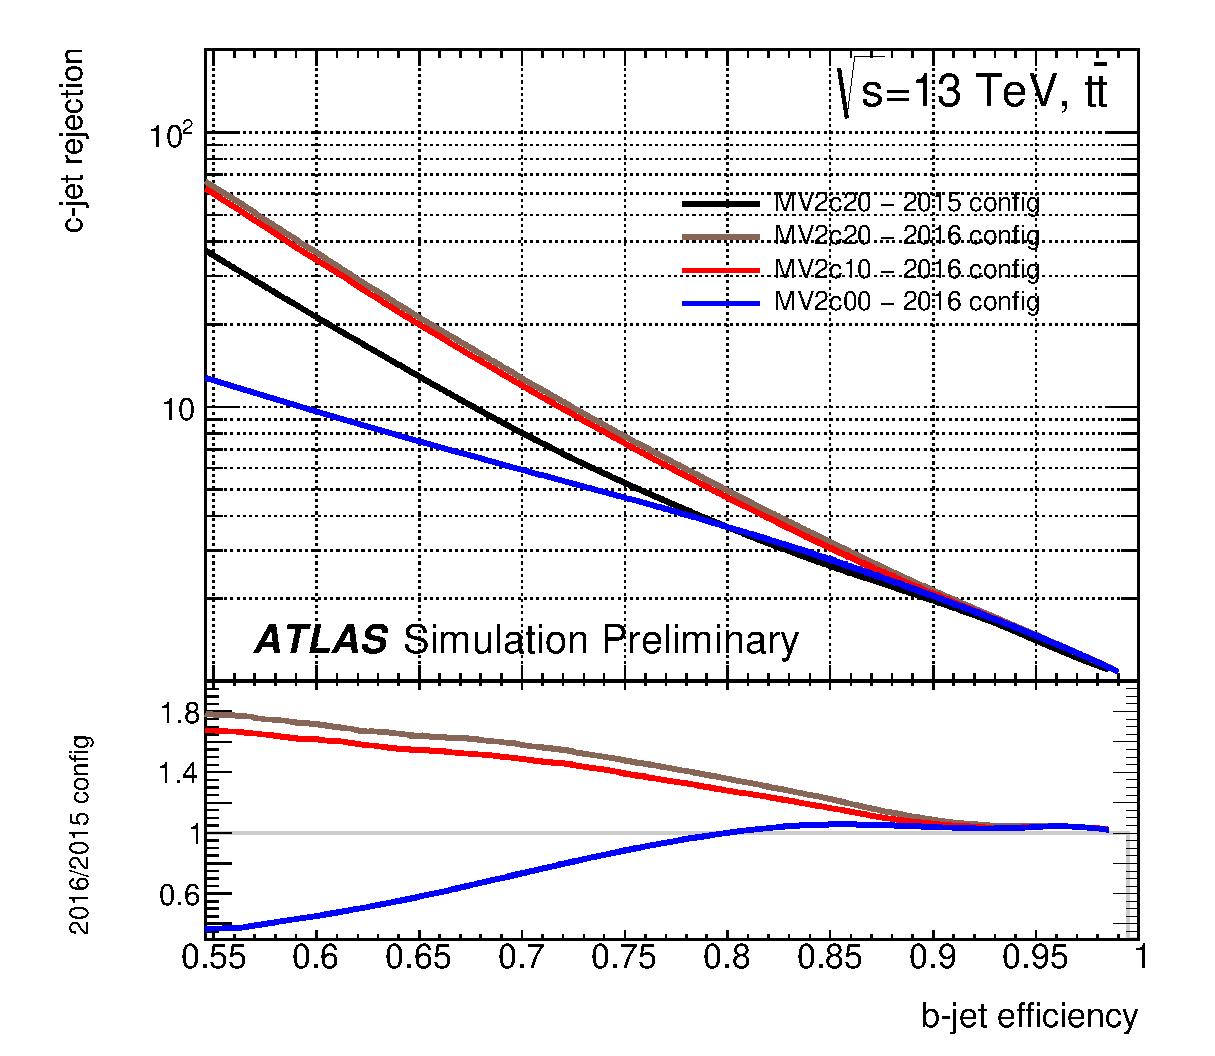
\includegraphics[width=0.9\textwidth]{figures/Objects/btagc.eps}
  \caption{}
  \label{}
\end{subfigure}
\captionsetup{width=0.85\textwidth} \caption{\small $b$-tagging efficiency compared to the (a) light-jet and (b) $c$-jet rejection for the MV2cxx algorithm, where xx represents the fraction of $c$-jets using in the training.}
\label{sec:obj:fig:mv2plot}
\end{figure}



Several operating points have been defined based on the average $b$-tagging efficiency of the algorithm on simulated $t\bar{t}$ events (see table \ref{tab:obj:jet:btag}). 
\begin{table}\footnotesize
\begin{center}
\begin{tabular}{|c|c|c|c|}
  \hline \hline
   $b$-jet efficiency [$\%$] & c-jet rejection & light-jet rejection & $\tau$-jet rejection \\
  \hline
  60 & 34 & 1538 & 184\\
  \hline
  70 & 12 & 381 & 55\\
  \hline
  77&6&134&22\\
  \hline
  85&3.1&33&8.2\\
 \hline \hline
\end{tabular}
\captionsetup{width=0.85\textwidth} \caption{\small The MV2c10 algorithm operating points and their performance. The $b$-jet efficiency is the average obtained for $b$-jets with $\pt>20$ $\gev$ from simulated $t\bar{t}$ events.}
\label{tab:obj:jet:btag}
\end{center}
\end{table}
The $70\%$ and $77\%$ operating points have been chosen for the analyses in this dissertation given the compromises in each of them between efficiency and rejection. Figure \ref{sec:obj:fig:btageff} shows the efficiency, obtained from the simulation, of the $70\%$ MV2c10 operating point for $b$-jet, c-jet and light-jets as a function of the jet $\pt$ and $|\eta|$. The $b$-tagging efficiency increases in the medium $\pt$ regime ($50<\pt<200$ \gev) where the identification of displaced vertices is more efficient, but at high $\pt$ ($>200$ \gev) starts dropping since the tracking reconstruction efficiency is worse due to merged-tracks effects. The mistag rate is more important for large $|\eta|$ values due to the worse track resolution.


\begin{figure}[h!]
\begin{subfigure}{0.5\textwidth}
  \centering
  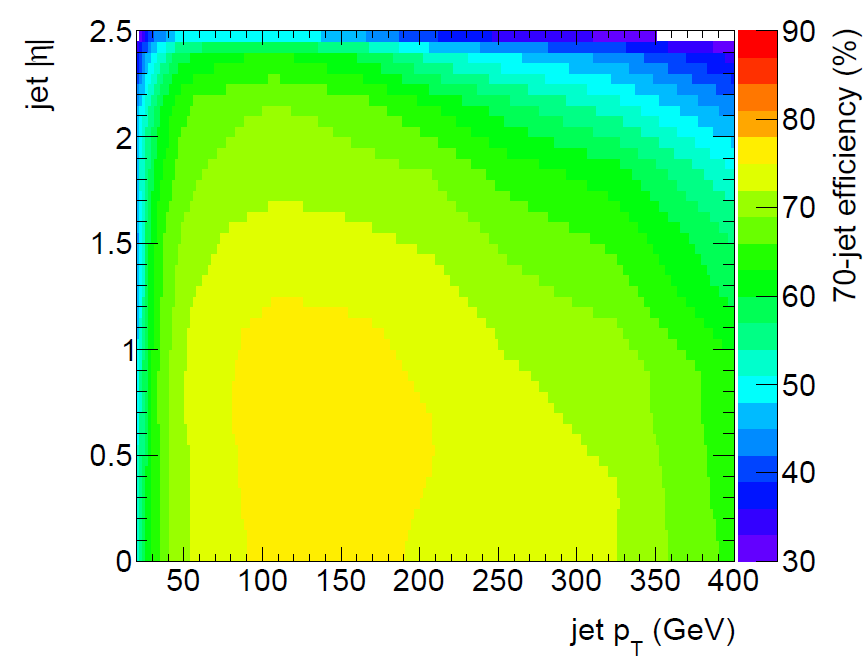
\includegraphics[width=0.9\textwidth]{figures/Objects/Eff_B.png}
  \caption{}
  \label{sec:obj:fig:beff}
\end{subfigure}
\begin{subfigure}{0.5\textwidth}
  \centering
  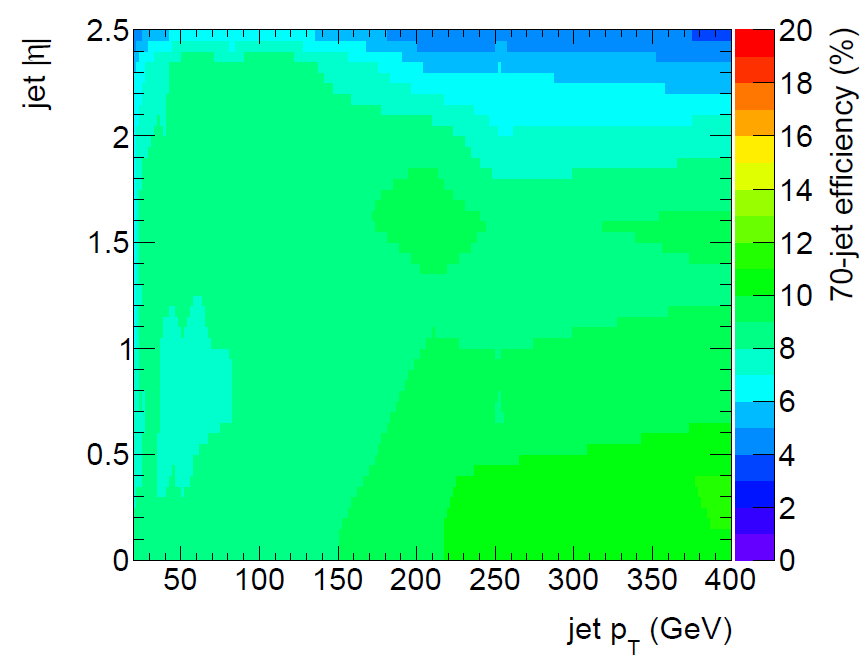
\includegraphics[width=0.9\textwidth]{figures/Objects/Eff_C.png}
  \caption{}
  \label{sec:obj:fig:ceff}
\end{subfigure}
\begin{center}
\begin{subfigure}{0.5\textwidth}
  \centering
  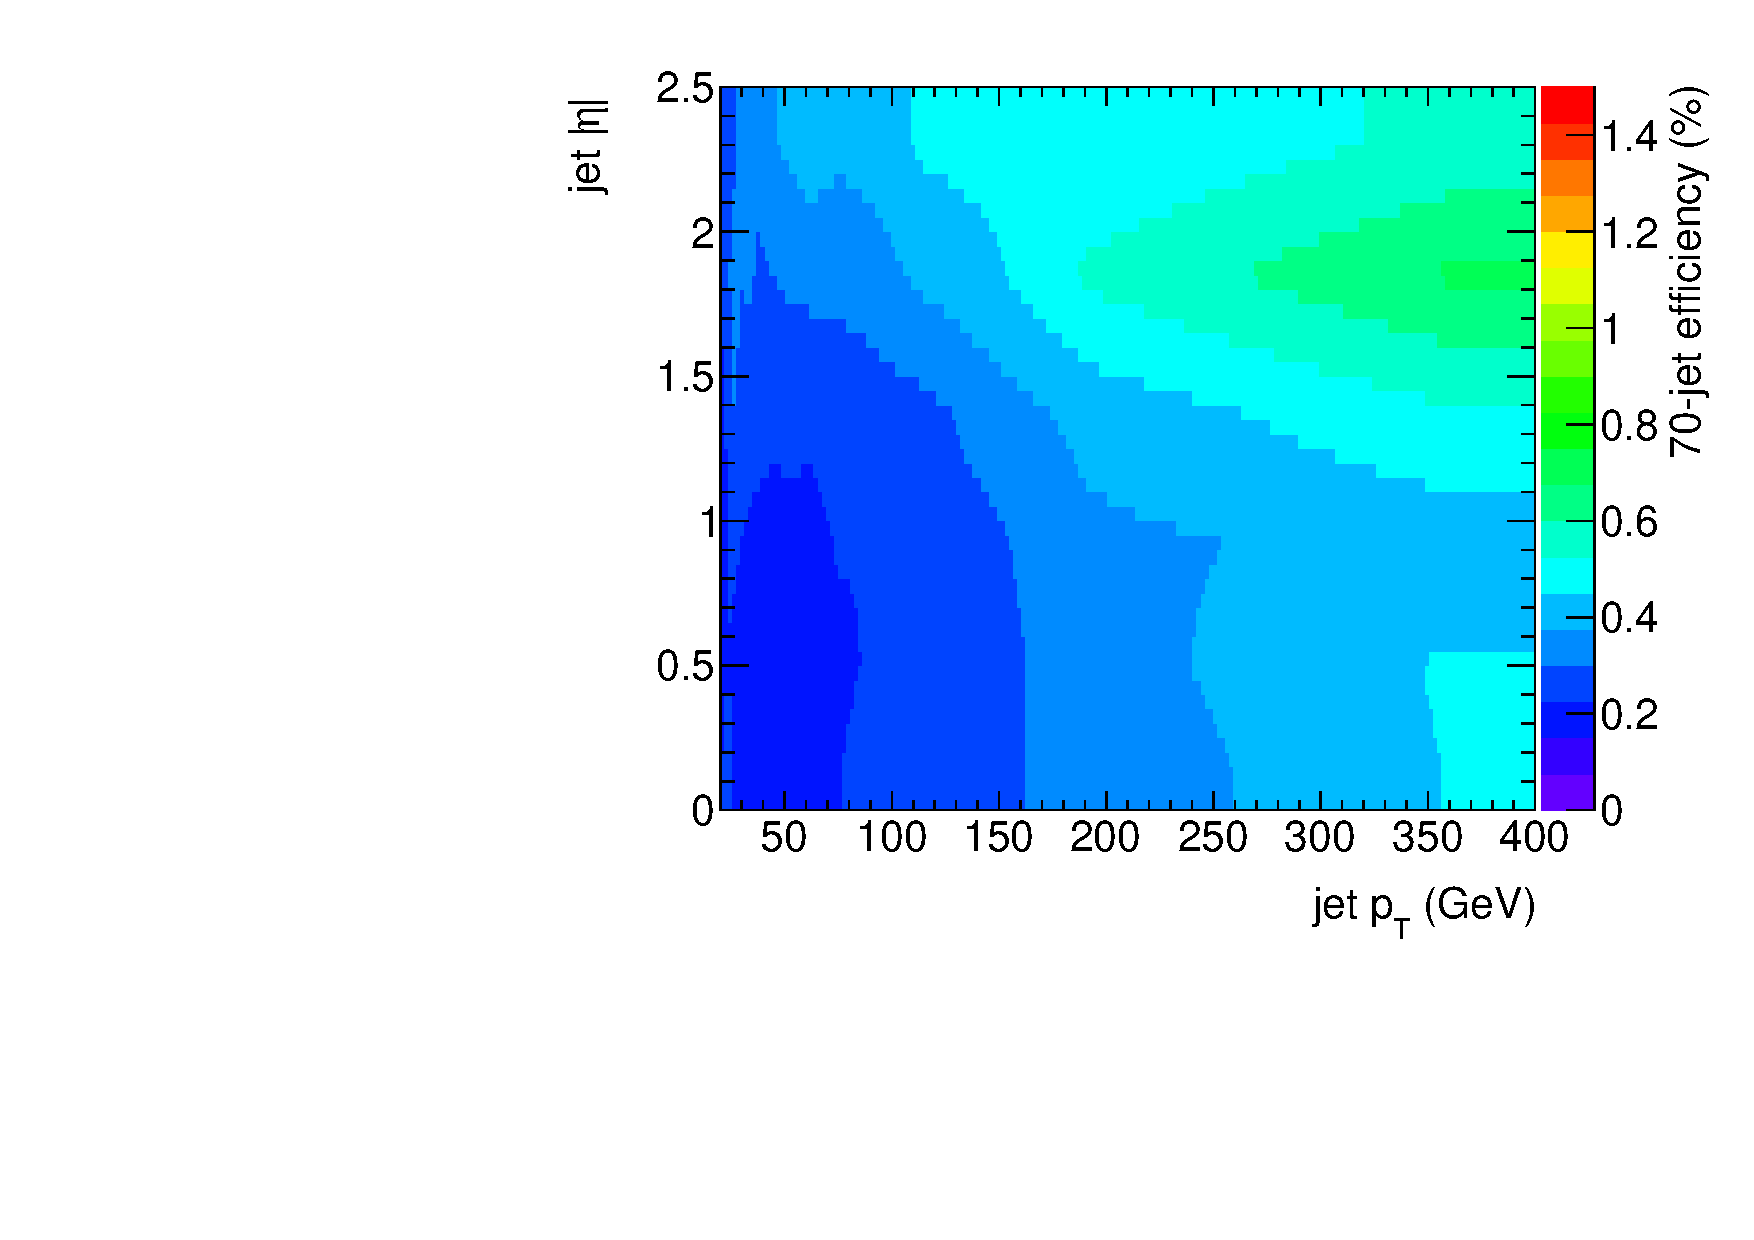
\includegraphics[width=0.9\textwidth]{figures/Objects/Eff_Light.png}
  \caption{}
  \label{sec:obj:fig:leff}
\end{subfigure}
\end{center}
\captionsetup{width=0.85\textwidth} \caption{\small $b$-tagging efficiency for the MV2c10 $70\%$ operating point as a function jet $\pt$ and $|\eta|$. Efficiencies are shown separately for (a) b-jets, (b) c-jets and (c) light jets from simulated $t\bar{t}$ events.}
\label{sec:obj:fig:btageff}
\end{figure}




\subsubsection[$b$-tagging calibration]{\boldmath{$b$}-tagging calibration}
In order to take possible differences between the MC simulation and real data into account, the $b$-tagging algorithms need to be calibrated in data. Several methods have been developed to measure the $b$-jet efficiency, the $c$-jet efficiency and the light-jet rate in data. The result is presented in terms of scale factors, ${\rm SF}= \epsilon_{\rm data}/\epsilon_{\rm MC} $. This allows correcting for mis-modeling by the MC simulation in the input variables used in the $b$-tagging algorithms.

The $b$-jet calibration used for the analyses in this dissertation is derived on a high-purity sample of $b$-jets that can be obtained from $t\bar{t}$ events with two oppositely-charged leptons in the final state \cite{BTagSF}. The calibration is based on a likelihood approach which uses correlated information from multiple jets in the event, and it achieves a precision of a few percent for jet $\pt$ ranging between 30 and 300 GeV. However a correct use in a physics analysis requires some care in order to avoid a re-use of the same data sample as well as double counting of systematic uncertainties. Since the chosen $t\bar{t}$ -based calibration has been derived using a dileptonic $t\bar{t}$  sample, no overlap of data events exists with analyses considering lower lepton multiplicities, such as the ones discussed in this dissertation.\par
The tagging calibration for $c$-quarks has been derived by reconstructing $D$-mesons within a jet from the decay chain $D^{*+}\to D^{0}\pi^{+}$ \cite{CTagSF}. The contamination of $D^{*+}$ mesons originating from $b$-hadron decays is identified fitting the pseudo-proper time distribution of the $D^{0}$ meson, and corrected for.\par For the mis-tag rate calibration the so-called ``negative tag'' method is used \cite{LTagSF}. 
Light-flavour jets are tagged as $b$-jets mainly because of the finite resolution of the inner detector and the presence of tracks from displaced vertices of long-lived particles or material interactions. For prompt tracks the distributions of the lifetime-signed impact parameter and of the signed decay length of vertices reconstructed using these tracks are expected to be symmetric. Therefore, the inclusive tag rate obtained by using negative impact-parameter tracks in the case of impact-parameter-based tagging algorithms, or by using negative decay-length secondary vertices in the case of secondary-vertex-based tagging algorithms, is expected to be a good approximation of the mistag rate due to resolution effects.\par 
Scale factors as a function of jet $\pt$ for $b$-, $c$- and light jets as extracted from the 2015 dataset are shown in figure \ref{sec:obj:fig:btagsf}.
\begin{figure}[h!]
\begin{subfigure}{0.5\textwidth}
  \centering
  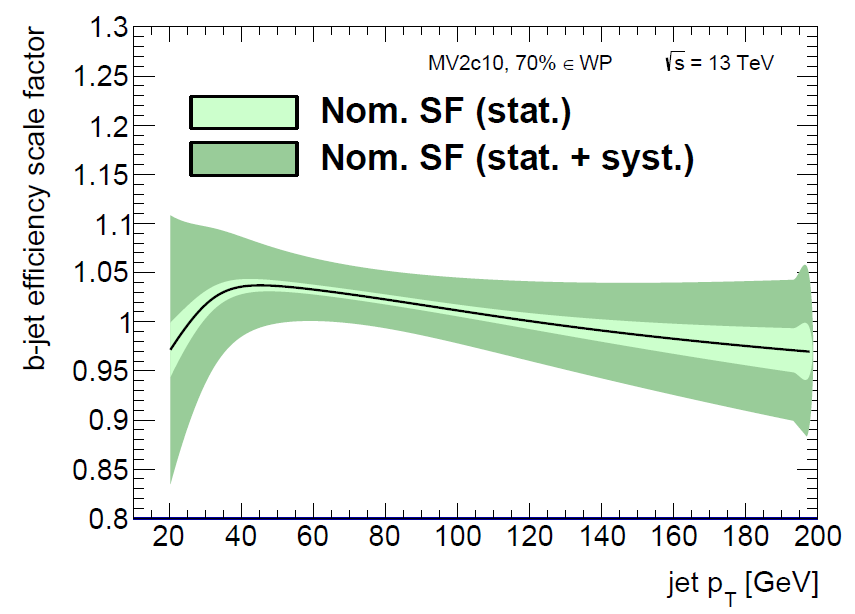
\includegraphics[width=0.9\textwidth]{figures/Objects/BSF.png}
  \caption{}
  \label{sec:obj:fig:bSF}
\end{subfigure}
\begin{subfigure}{0.5\textwidth}
  \centering
  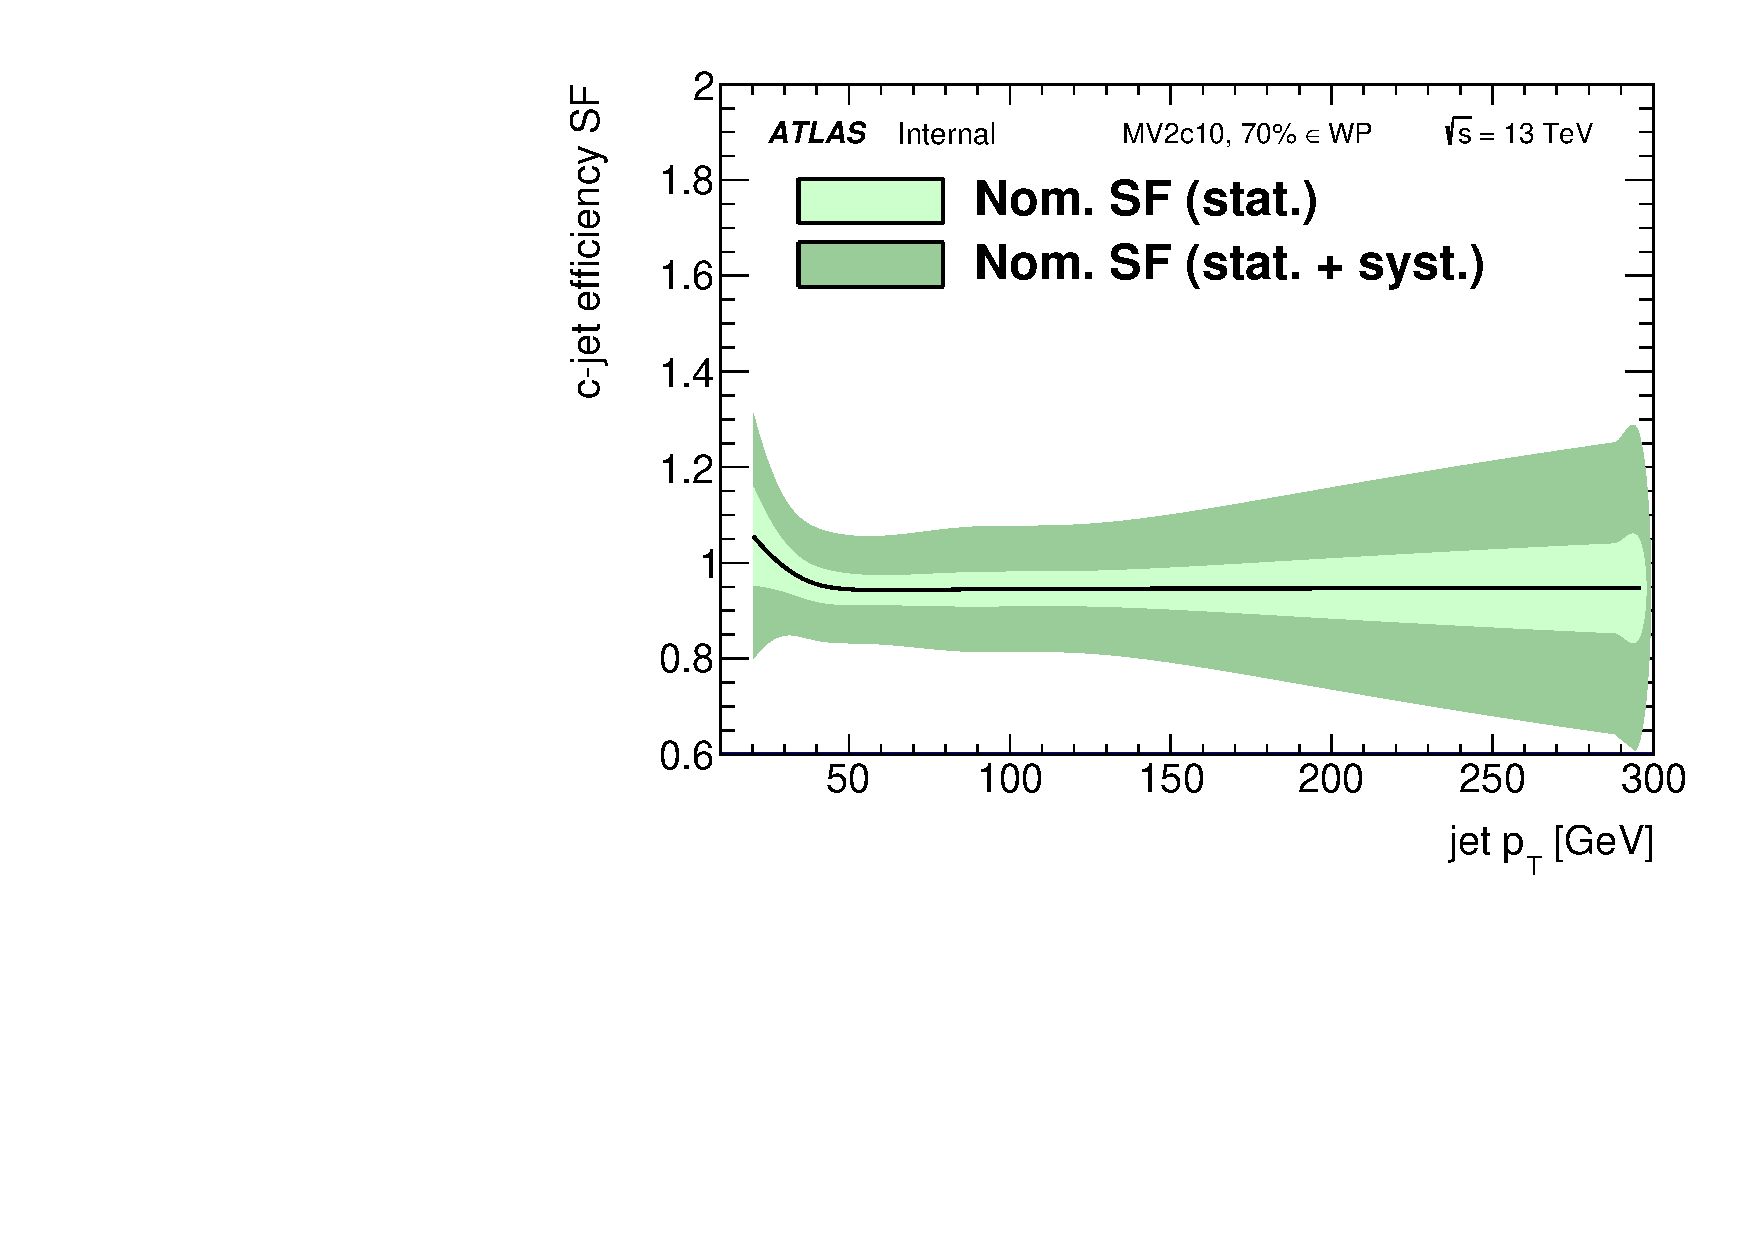
\includegraphics[width=0.9\textwidth]{figures/Objects/CSF.png}
  \caption{}
  \label{sec:obj:fig:cSF}
\end{subfigure}

\begin{subfigure}{0.5\textwidth}
  \centering
  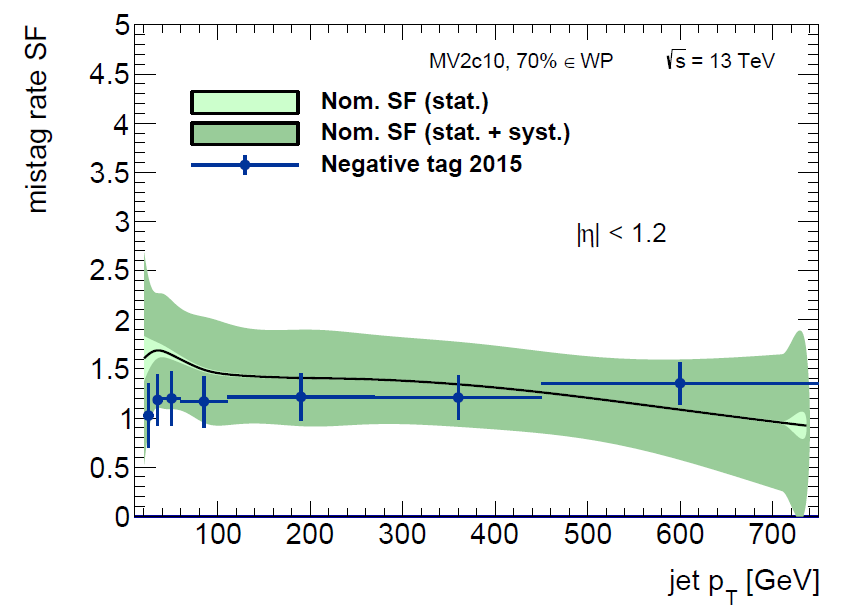
\includegraphics[width=0.9\textwidth]{figures/Objects/LSFc.png}
  \caption{}
  \label{sec:obj:fig:lSFc}
\end{subfigure}
\begin{subfigure}{0.5\textwidth}
  \centering
  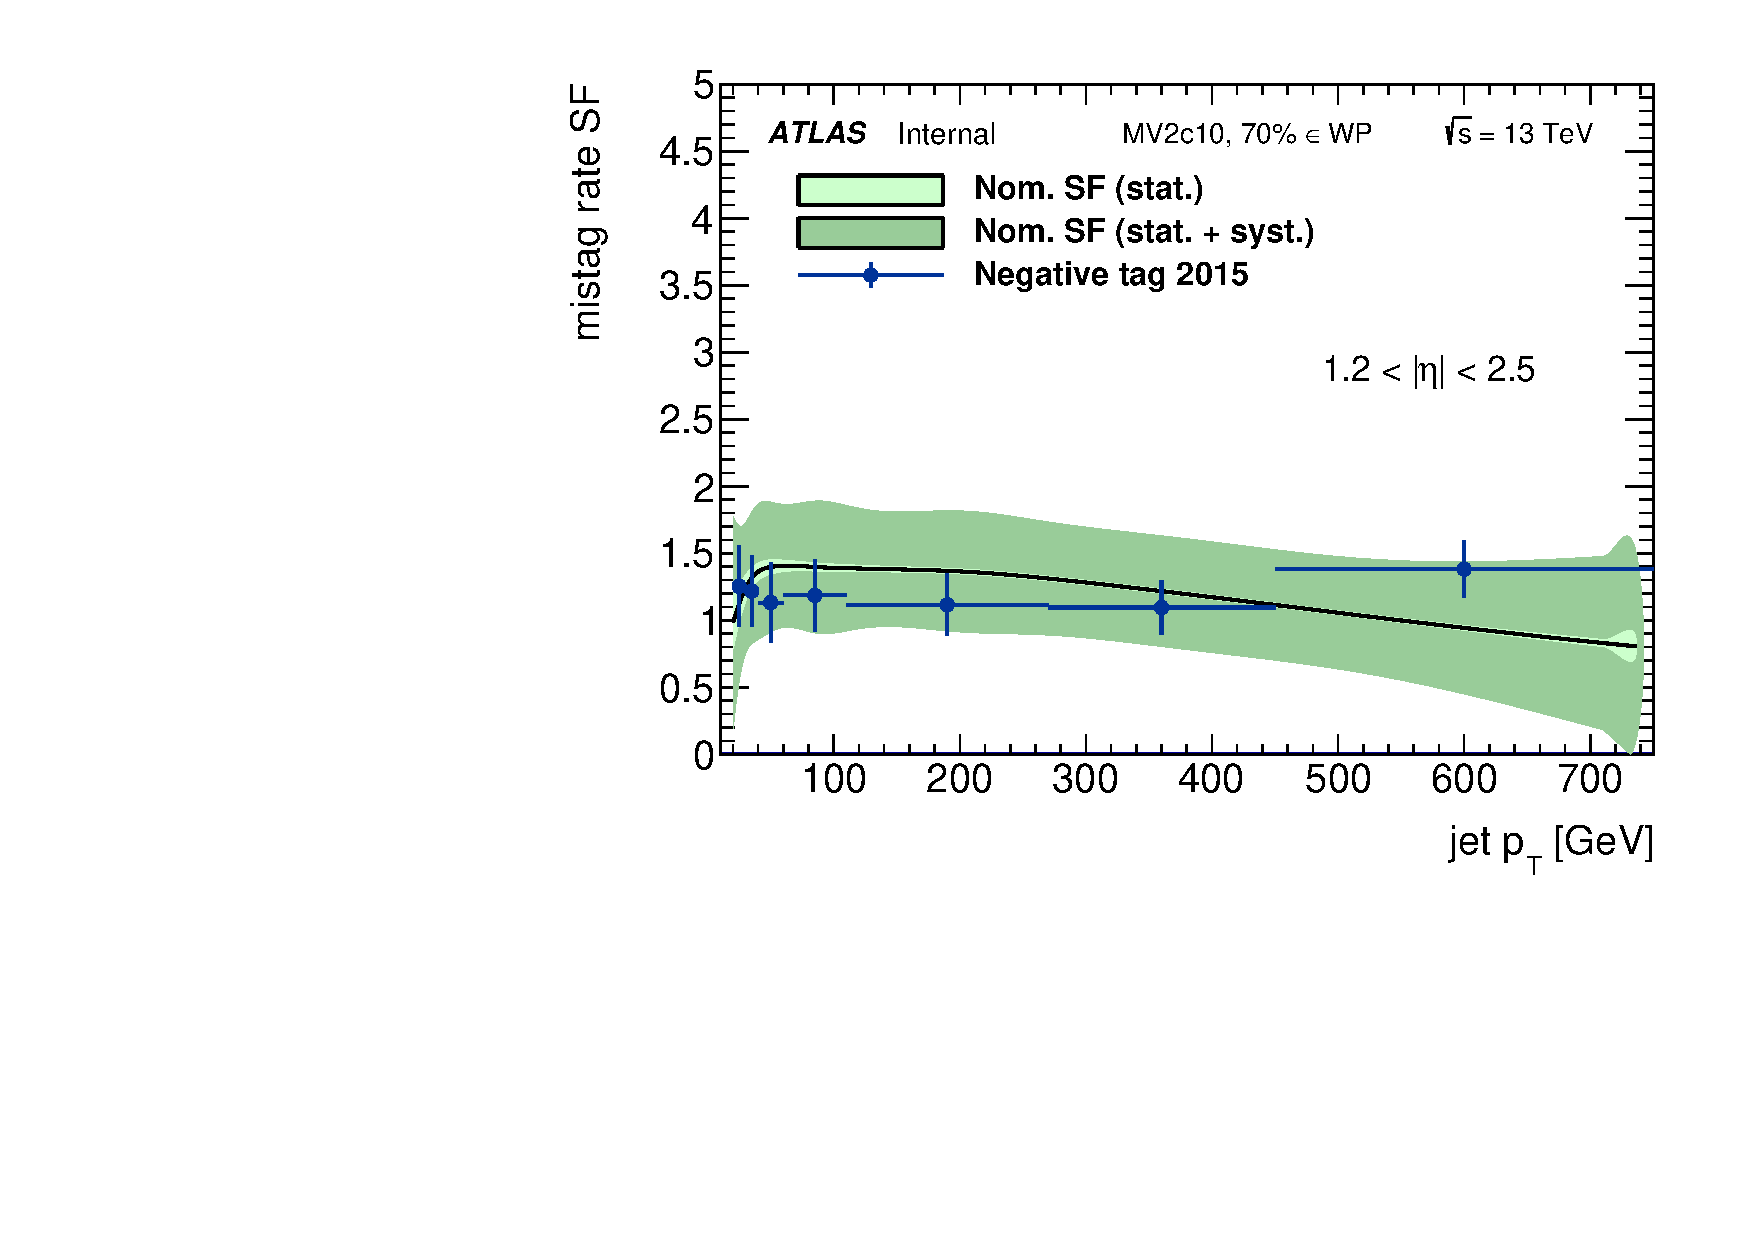
\includegraphics[width=0.9\textwidth]{figures/Objects/LSFf.png}
  \caption{}
  \label{sec:obj:fig:lSFf}
\end{subfigure}

\captionsetup{width=0.85\textwidth} \caption{\small Data/MC scale factors for the tagging efficiency of (a) $b$-jets, (b) $c$-jets, and (c and d) light jets with the $70\%$ MV2c10 operating point. Total uncertainty are shown as well as the statistics component. Scale factors are measured as a function of jet $\pt$ and, in case of the light-jet mistag rate, the result for two different $|\eta|$ bins are shown.}
\label{sec:obj:fig:btagsf}
\end{figure}
The scale factors are applied to MC samples as event weight corrections. For each jet tagged by the $b$-tagging algorithm, a weight equal to the $b$-tagging SF of the corresponding jet flavour is considered. If a jet fails the $b$-tagging criterion, a weight corresponding to $(1-{\rm SF}\times\epsilon_{\rm MC})/(1-\epsilon_{\rm MC})$ is assumed. The individual jet weights for all the selected jets are multiplied in order to obtain an event-level weight. The determination of the $b$-tagging scale factors is affected by multiple systematic uncertainties. In order to propagate those into the scale factors in a manageable way a reduction in terms of 23 independent nuisance parameters through a diagonalisation method is used. A total of five eigenvectors are considered to describe the systematic uncertainties related to the $b$-tagging calibration. The same procedure is performed to derive four (fourteen) eigenvectors on the $c$-tagging (mistag) calibration. An additional uncertainty is included due to the extrapolation of the $b$-, $c$-, and light-jet-tagging scale factors for jets with $\pt$ beyond the kinematic reach of the data calibration samples used: $\pt>300 \,\gev$ for $b$- and $c$-jets, and $\pt>750\,\gev$ for light-jets. Finally, in absence of a direct measurement in data, for $\tau$-jets the $c$-jet SF is used, and a related extrapolation uncertainty (referred to as $c \to \tau$ extrapolation) is assigned.

